%%%%%%%%%%%%%%%%%%%%%%%%%%%%%%%%%%%%%%%%%%%%%%%%%%%%%%%%%%%%%%%%%%%%%%%%%%%
% filename    : sp.tex
% author      : 
%%%%%%%%%%%%%%%%%%%%%%%%%%%%%%%%%%%%%%%%%%%%%%%%%%%%%%%%%%%%%%%%%%%%%%%%%%%

% BUGFIX: Save LaTeX kernel version of \@xfloat
\makeatletter
\let\my@xfloat\@xfloat
\makeatother

% use ateneo de naga etd class (actually modified virginia tech's etd class)
\documentclass[oneside]{etd}

% BUGFIX: Create a modified copy of \@xfloat using the kernel definition
\makeatletter
\def\@xfloat#1[#2]{
	\my@xfloat#1[#2]%
	\def\baselinestretch{1}%
	\@normalsize \normalsize
}
\makeatother

% use these packages
\usepackage{tabularx}
\usepackage{booktabs}
\usepackage{graphicx}
\usepackage{amssymb}
\usepackage{textcomp}
\usepackage{gensymb}
\usepackage{url}
\usepackage{hyperref}
\usepackage{doi}
\usepackage{latexsym}
\usepackage{amsmath}
%\usepackage[lineno5,noindent]{lgrind}
%\usepackage{rotating} 
%\usepackage{makeidx}
%\usepackage{stmaryrd}
\usepackage{float}
\usepackage{subcaption}
%\usepackage{cite}
%\usepackage{moreverb}
%\usepackage{pictexwd,dcpic}
\usepackage{algorithm,algorithmic}
\renewcommand{\algorithmicrequire}{\textbf{Input:}}
\renewcommand{\algorithmicensure}{\textbf{Output:}}
\usepackage{tikz}
\usetikzlibrary{positioning,calc}

\usepackage{listings}
\definecolor{cppred}{rgb}{0.6,0,0} % for strings
\definecolor{cppgreen}{rgb}{0.25,0.5,0.35} % comments
\definecolor{cpppurple}{rgb}{0.5,0,0.35} % keywords
\definecolor{cppdocblue}{rgb}{0.25,0.35,0.75} % doc
 
\lstset{language=C++,
basicstyle=\linespread{0.8}\ttfamily\small,
keywordstyle=\color{cpppurple}\bfseries,
stringstyle=\color{cppred},
commentstyle=\color{cppgreen},
morecomment=[s][\color{cppdocblue}]{/**}{*/},
numbers=left,
numberstyle=\tiny\color{black},
% stepnumber=2,
numbersep=10pt,
tabsize=4,
showspaces=false,
showstringspaces=false}

\graphicspath{{figures/}{./}}

%\renewcommand{\floatpagefraction}{0.8}

\makeindex

%%%%%%%%%%%%%%%%%%%%%%%%%%%%%%%%%%%%%%%%%%%%%%%%%%%%%%%%%%%%%%%%%%%%%%%%%%%

\title{MARQ: A Multi-Agent Rainbow Deep Q-Networks Framework using AAREN for Mastering Imperfect Information Games}
\department{Computer Science}
\BSthesis % options: \BSthesis \BSproject \BShonors \Mdegree \MSdegree \PhDdegree
\degreemonth{September 5}  % date of final defense
\degreeyear{2025}

\twostudents % options: \onestudent \twostudents \threestudents \fourstudents
{James Gabriel P. Mabagos}
{Mark Lawrence M. Quibot}


\studentsheader
{Mabagos and Quibot}

\twodegrees % options: \onedegree \twodegrees \threesdegrees \fourdegrees
{Computer Science}
{Computer Science}

\advisor
{Marianne A. Tolentino}
\threemembers
{Estrella H. Montealegre}
{
Michelle Elija B. Santos}
{Ian Peter L. Lastimosa}
\deanandchair
{Joshua C. Martinez MIT }
{Lowie Vincent S. Bisana MIT}

\keywords{Imperfect Information, DQN, Multi-Agent}

\begin{document}

%edit etd.cls to accommodate lesser number of proponents
\maketitle
\makerecomm
\makeacceptance
\makedeclaration

%%%%%%%%%%%%%%%%%%%%%%%%%%%%%%%%%%%%%%%%%%%%%%%%%%%%%%%%%%%%%%%%%%%%%%%%%%%
%                    ABSTRACT/EXECUTIVE SUMMARY                           %
%%%%%%%%%%%%%%%%%%%%%%%%%%%%%%%%%%%%%%%%%%%%%%%%%%%%%%%%%%%%%%%%%%%%%%%%%%%

% can use execsummary or abstract
\begin{abstract}
This research presents MARQ, a Multi-Agent Rainbow Deep Q-Networks, designed to master imperfect information games through the board game Stratego. MARQ leverages a Deep Recurrent Q-Network (DRQN) architecture and league-based self-play training to address the large state space of Stratego and hidden information challenges. The architecture integrates an Attention as Recurrent Neural Network (AAREN) module that produces learned embeddings from observed opponent behavior, enabling implicit piece identity inference through end-to-end training. The system employs Distributional Reinforcement Learning with Noisy Networks to balance strategic unpredictability and stability. The methodology involves developing a game environment and training the AI agent through multi-channel state representations, incorporating AAREN-generated embeddings for hidden information modeling and weighted piece values computed through systematic power analysis to optimize decision making under uncertainty. A structured participant study introduces enthusiasts without prior Stratego experience to create a synchronized learning environment, combining quantitative metrics including win rate percentage, average game length, and decision-making speed, with qualitative usability assessments across performance, reliability, and applicability dimensions. Through this study MARQ aims to deliver strategic decisions comparable to human opponents.
\end{abstract}

\include{misc/dedication}
\include{misc/acknowledgements}

\begingroup
\renewcommand*{\addvspace}[1]{}
\tableofcontents
\listoffigures
\listoftables
\endgroup

\beginbody
\pagenumbering{arabic}

\chapter{Introduction}
\section{Project Context}
Games have a history of being a metric for how Artificial Intelligence (AI) progresses and performs in the current time \cite{StudeGame}. Many real-world problems, from military tactics to multiplayer games, require intelligent decision-making in environments where all information is not available. A common example is a feature found in many multiplayer games known as the "fog of war"  \cite{FogofWar}, where the game environment is not fully revealed, which makes it an example of an imperfect information game \cite{National}. Imperfect information games create a scenario where players develop unconventional strategies without having full knowledge of the game's environmental state \cite{FogofWar}. Solving these kinds of problems and determining the optimal strategy remains a significant challenge for Artificial Intelligence \cite{GeneralGame}.

This study focuses on mastering imperfect information games through Multi-Agent Reinforcement Learning (MARL) with Deep Q-Networks (DQN). In MARL, multiple agents learn and adapt in the same environment, making each decision based on its own observations and rewards \cite{MARLCOMP, MARLCHALL}. With DQN, the agents can utilize deep neural networks to approximate the Q-function that maps state-action pairs for the expected reward. With all of these together, this study introduces MARQ (Multi-Agent Rainbow Deep Q-Networks), a framework to solve imperfect information games. This approach is suited well for Stratego, where these agents are trained to compete against each other, developing strategies through repeated experience, even though information is lacking about the opponent's setup or the environment's full state. 


\section{Purpose and Description}
This research aims to evaluate whether Multi-Agent Reinforcement Learning (MARL) with Deep Q-Networks (DQN) can be used to develop intelligent agents capable of mastering imperfect information games. By focusing on the limited information available to players in environments such as the board game Stratego, this study seeks to address the challenge of making decisions under uncertainty while incorporating strategic planning. Although existing tools for Stratego provide some analytical support, they are often limited in fostering deeper reasoning about the game’s tactical complexities.


To advance beyond these limitations, this research seeks to provide an algorithmic foundation for future analytical systems while also emphasizing the development of critical thinking in solving imperfect information games. By modeling adaptive strategies and reasoning under uncertainty, the study highlights how artificial intelligence can mirror and enhance human-like logical reasoning, offering valuable insights for both game analysis and broader decision-making domains.
\subsection{Research Questions}
This study is guided by three main research questions:

\begin{enumerate}
   
    \item How effective is the AI agent in adapting to hidden information and different strategies?
    \item To what extent does the trained AI agent’s performance compare against human players and other AI opponents in Stratego?
    \item How does the use of Stratego as a research platform contribute to advancing studies in imperfect information multi-agent reinforcement learning?
\end{enumerate}

\section{Objectives}
The main objective of this study is to develop and evaluate Multi-Agent Reinforcement Learning with Deep Q-Networks for learning appropriate strategies in an imperfect information game, where the agents operate under hidden state variables to improve decision-making, adaptability, and strategic reasoning against both human and AI opponents. This can be achieved through the following:
\begin{itemize}
    \item Introduction of Stratego to the community
    \item Design and implement a game environment for Stratego
    \item Build and implement a training model using Multi-Agent Reinforcement Learning with Deep Q-Networks and AAREN.
    \item Train and optimize the AI agent to respond to varying game states, hidden information, and opposing strategies.
\end{itemize}

\section{Scope and Limitation}

The study is limited to the development of an AI agent for imperfect information games, Stratego being the test environment. The scope includes the design and implementation of Stratego as a game environment, the development of a training framework using Multi-Agent Reinforcement Learning (MARL) with Deep Q-Networks (DQN) using AAREN, and the training and optimization of the AI agent to adapt to differences in game states. The evaluation of the agent's performance would primarily be on Stratego's environment. The trainings are limited to the personal devices of the researchers and would not rely on cloud-based computing resources. Since the AI is going to learn alongside the community the player and AI head-to-head will be analyzed mostly qualitative. The goal will be achieving the same human critical thinking in the model.

\section{Significance of the Study}
The development of MARQ addresses limitations in current imperfect information game AI, where existing systems either require large computational resources or employ model-free approaches that limit strategic depth.
MARQ's significance lies in its explicit opponent modeling through AAREN and probabilistic belief states, and hybrid DQN architecture that balances strategic depth with computational tractability. The synchronized learning evaluation framework provides insights into AI adaptability against improving human opponents, with implications extending beyond gaming to domains characterized by incomplete information and strategic interaction, including cybersecurity, financial trading, and strategic planning.

\section{Definition of Terms}

\noindent\textbf{AAREN} \\
Attention a recurrent neural network, a model that integrates the sequential processing of RNNs with the parallel efficiency of Transformers, designed for tasks such as event forecasting and classification. \\[6pt]

\noindent\textbf{Alpha-Beta Pruning} \\
A search algorithm that explores possible moves in a game tree while pruning branches that cannot affect the final decision, making the search process more efficient. \\[6pt]

\noindent\textbf{Counterfactual Regret Minimization (CFR)} \\
An iterative algorithm that approximates Nash equilibrium by minimizing regret, widely applied in imperfect information games such as Poker and Stratego. \\[6pt]

\noindent\textbf{Deep Q-Networks (DQN)} \\
A reinforcement learning algorithm that combines Q-learning with deep neural networks, enabling agents to approximate optimal decision-making in complex environments. \\[6pt]

\noindent\textbf{Fog of War} \\
A game mechanic used in strategy games that conceals parts of the map or opponent actions, requiring players to utilize prediction and information-gathering strategies to reduce uncertainty. \\[6pt]

\noindent\textbf{Imperfect Information Games} \\
Games where players have incomplete knowledge of the current game state, requiring them to make strategic decisions under uncertainty (e.g., Stratego, Poker, Multiplayer Online Battle Arenas). \\[6pt]

\noindent\textbf{ Knowledge-Limited Unfrozen Subgame Solving(KLUSS)} \\
Knowledge-Limited Unfrozen Subgame Solving (KLUSS) is an advancement in search algorithms for imperfect-information games. KLUSS builds on the earlier Knowledge-Limited Subgame Solving (KLSS) method, which simplified computation by removing irrelevant states and freezing certain strategies. \\[6pt]

\noindent\textbf{Long Short-Term Memory (LSTM)} \\
A variant of RNN designed to capture long-term dependencies in sequential data while mitigating the vanishing gradient problem. \\[6pt]

\noindent\textbf{Multi-Agent Reinforcement Learning (MARL)} \\
An extension of reinforcement learning in which multiple agents interact within the same environment, learning coordinated or competitive strategies through simultaneous training. \\[6pt]

\noindent\textbf{Nash Equilibrium} \\
A game-theoretic concept where no player can gain an advantage by unilaterally changing their strategy, often used as a benchmark for decision-making in imperfect information games. \\[6pt]

\noindent\textbf{Perfect Information Games} \\
Games in which all players have complete knowledge of the current game state and available moves, such as Chess and Go. \\[6pt]

\noindent\textbf{Proximal Policy Optimization (PPO)} \\
A reinforcement learning algorithm that optimizes policies through probability ratio clipping, often compared to DQN in performance within gaming environments such as VizDoom. \\[6pt]

\noindent\textbf{Recurrent Neural Network (RNN)} \\
A type of neural network designed to process sequential data by maintaining memory of previous inputs, useful in imperfect information games for recalling past moves or revealed information. \\[6pt]

\noindent\textbf{Reinforcement Learning (RL)} \\
A machine learning paradigm where agents learn optimal strategies through trial-and-error interactions with the environment, guided by rewards and penalties. \\[6pt]

\noindent\textbf{Stratego} \\
A two-player strategy board game characterized by hidden information and asymmetric piece abilities, where the objective is to capture the opponent’s flag or render them immobile. \\[6pt]

\noindent\textbf{Student of Games (SoG)} \\
A unified AI framework combining self-play learning, strategic search, and game-theoretic reasoning, designed to handle both perfect and imperfect information games. \\[6pt]

\noindent\textbf{Vanishing Gradient} \\
The vanishing gradient problem is basically as in the name, vanishing gradient, as color in a gradient, the message in this case starts strong and gradually fades away when it passes through each layer, making the learning weak or close to zero.\\[6pt]

\chapter{Review of Related Literature}
\section{Artificial Intelligence in Imperfect Information Games}
Games can be classified as an imperfect information game by having incomplete information about the current game state for both players \cite{StudeGame, 2509_03682v1}. An example would be in MOBAs (Multiplayer Online Battle Arena), the fog of war mechanic hides portions of the map, including objectives and enemy positions, from both teams. By placing a tool, such as a ward in League of Legends or an observer in Dota 2, the player gains a temporary vision in the map for strategic planning \cite{WARDS}. This feature engages players to create strategic reasoning under certainty, utilizing prediction, coordination, and resource management to gain informational advantages over opponents. Games have a history of being a metric on how AI progresses and performance in the current time \cite{StudeGame, GamePer}. The case is the same for both perfect information and imperfect information games \cite{StudeGame}. For perfect information games, like chess, they primarily use Alpha-Beta pruning, a search algorithm that uses trees to explore possible chess moves and prunes the branches that will not affect the final decision \cite{alphabeta}. In imperfect information games, a search algorithm like Alpha-Beta Pruning would be difficult to implement because the algorithm is made for perfect information games \cite{alphabe}. A popular algorithm that is used in imperfect information games would be Monte Carlo Tree Search with Reinforcement Learning because MCTS has integration with neural network systems like AlphaZero \cite{AIAgent, AlphaStratego}. In terms of reinforcement learning, the training focuses on trial and error to provide the best possible decision \cite{comprel}. Continuing development of AI algorithms in imperfect information games advances our understanding of decision-making under uncertainty and promotes strategic planning.


\subsection{Student of Games}
A unified learning algorithm that can support both perfect information and imperfect information is Student of Games. Combining self-play learning, strategic search, and principles from game theory \cite{StudeGame}. SoG achieved strong performance in Chess and Go in perfect information games and in imperfect information games like heads-up no-limit Texas hold ’em poker, and defeated the state-of-the-art agent in Scotland Yard. When comparing to MARL, SoG supports and has been tested in both game types and uses game theoretic reasoning, which computes or approximates the Nash equilibria. MARL with DQN uses trial and error learning and self-play learning, which relies on the exploration of the environment. MARL has also been tested in complex video games \cite{2509_03682v1}, unlike SoG, which has not been tested in video games.

\subsection{Deep Q-Networks and Dueling Architectures}
Deep Q-networks (DQN) and their variants have become a standard framework for decision-making in complex environments with high-dimensional observations. Hessel et al. (2021) combined several independent improvements to DQN—such as double Q-learning, prioritized replay, dueling networks, and noisy nets—into a unified agent called Rainbow, demonstrating state-of-the-art performance on competitive benchmarks \cite{RainbowJMLR2021}. This demonstrates that carefully integrating architectural and algorithmic improvements can substantially improve both data efficiency and final performance in value-based deep RL.

A key architectural component of Rainbow is the dueling network architecture, proposed by Wang et al. (2016) and detailed in modern surveys \cite{RainbowJMLR2021, DRLImperfectInfo2023}. This design splits the Q-function into a state-value stream and an advantage stream. This split allows the network to generalize across actions and improves policy evaluation, particularly in environments with many similar-valued actions. Our MARQ model builds on this idea by feeding the shared ResNet-based representation into dueling value and advantage streams, which is particularly beneficial in board games where many positions have similar strategic value.


\subsection{Multi-Agent Reinforcement Learning}
Reinforcement Learning can solve complex problems through trial and error, by learning from the environment to be able to provide optimal decisions \cite{2509_03682v1}. This can be the case for Single-Agent Reinforcement Learning(SARL). SARL has its limits in solving many real-world problems. Multi-Agent Reinforcement Learning(MARL) was introduced as a solution for the challenges of SARL, by having multiple agents in an environment that interact with each other, the decisions they could make would be optimized \cite{2509_03682v1}. Optimized, meaning that these agents go through trial and error together to make the best decision given the reward. As for the implementation of this in Stratego, two agents would compete with each other to know the optimal decisions given the environment, which has imperfect information and opposing strategies.
As MARL has its advantages, it also has challenges. The first would be Non-Stationarity, and the second is scalability, as for non-stationarity, each agent learns simultaneously, meaning the environment constantly changes \cite{MARLCHALL}. For scalability, as more agents are being used, the computational power rises, making it expensive \cite{CFRMIX, MARLCHALL}. Recent work on Ataraxos demonstrates that these challenges can be addressed through careful regularization: by constraining policy updates toward both exploratory (uniform) and stable (target network) anchors with time-varying coefficients, agents can achieve superhuman performance in complex imperfect-information games while maintaining training stability \cite{Ataraxos2025}.


\subsection{Counterfactual Regret Minimization}
Counterfactual Regret Minimization(CFR) is an iterative algorithm that approximates the Nash equilibria commonly used on imperfect information games like poker and Stratego \cite{CFRMIX,xu2024dynamic}. The Nash equilibria are what CFR approximates to make the best possible decision with minimal regret. Regret in this scenario is the what-ifs of the algorithm if the algorithm chooses the other decision. For CFR to make decisions, it repeatedly minimizes regret to approximate the Nash equilibria \cite{CFRMIX}. Other works have made variations of the base CFR, showing improved convergence rate, but require a significant amount of effort by researchers. A framework is proposed named AutoCFR, instead of relying on manually crafted algorithms, it automatically designs new CFR variants using an outer loop to search over algorithm designs and an inner loop to test them on equilibrium finding tasks \cite{xu2022autocfr}. 

\subsection{Opponent Modeling in Imperfect-Information Games}
In imperfect-information games, an agent’s optimal strategy depends not only on the environment but also on the behavior of the opponent. Classical opponent modeling often builds models from observed action frequencies, and computes best responses in a game-theoretic framework. Li et al. (2024) formalize opponent-model search in games with incomplete information, providing algorithms to compute optimal or robust strategies given various forms of opponent knowledge \cite{li2024opponent}.

In the deep RL setting, modern approaches encode observations of opponents directly into the network trunk, jointly learning a policy and an opponent model without explicitly predicting actions \cite{DRLImperfectInfo2023}. This shows that learning implicit opponent representations from interaction traces can be more effective than handcrafted models, especially in high-dimensional state spaces. Our AAREN module follows this tradition of implicit opponent modeling but is specialized to board games with hidden piece identities. Instead of maintaining explicit probability distributions over opponent piece types, AAREN aggregates observed opponent action sequences into dense embedding vectors. These vectors are then concatenated as additional input channels to the Q-network, allowing the agent to reason about the opponent’s likely pieces and strategy in a learned representation space.




\section{RNN}
Recurrent Neural Network is a type of Neural Network designed to process sequential data. Unlike common Neural Networks, RNNs have a memory because the information passed to the next step is based on the memory from the previous step. RNN can be applied to imperfect information games such as Stratego because of its memory. By using the memory to remember the pieces that have been revealed, the decision could be optimized \cite{AIAgent}.

\subsection{History Aggregation and State Representation Learning}
Learning from histories is a central challenge in partially observable and non-Markovian environments. Wang et al. (2026) show how to systematically construct non-Markovian decision processes by aggregating interaction histories into state representations, providing an effective way to add temporal dependencies into RL \cite{wang2026history}. By explicitly modeling history via learned aggregators, an agent can better handle complex temporal structures.

More broadly, representation learning for RL has explored the use of embeddings to generalize across states and goals. Echchahed and Castro (2025) highlight in their survey that separating dynamics from rewards allows policies to be transferred across tasks through learned representations \cite{echchahed2025srl}. Our AAREN embeddings can be viewed as a form of history-dependent state representation that encodes the opponent’s action history into a compact vector to augment the board state. This approach is tailored to the specific structure of imperfect-information board games where opponent behavior reveals hidden state. By learning these embeddings jointly with the Q-network, we avoid the need to handcraft belief distributions and instead let the network infer implicit piece identities from observed behavior.
\subsection{LSTM}
Long Short-Term Memory is a popular RNN variant that has the capabilities of RNN but also processes data with long-term dependencies \cite{ALSELWI2024102068}. LSTM mitigates the vanishing gradient problem that RNN faces. The vanishing gradient problem is basically as in the name, vanishing gradient, as color in a gradient, the message in this case starts strong and gradually fades away when it passes through each layer, making the learning weak or close to zero. LSTM can be used to solve imperfect information games because of its capability to process data with long-term dependencies while having the memory of RNN.
\subsection{Aaren}
Aaren, known as Attention as a recurrent neural network, combines the parallel training efficiency of Transformers with the streaming update efficiency of RNNs \cite{Aaren}. Aaren, like transformers, can be trained in parallel as well as RNN, can process sequential data with memory. In the study, Aaren was tested in event forecasting, time series forecasting, and classifications. Aaren achieved similar accuracy to Transformers but was more time and memory-efficient.

\subsection{Residual Networks and Self-Attention in Board Games}
Residual networks (ResNets) have become a common backbone in modern board-game RL systems. AlphaZero-style agents for Go, chess, and Stratego use a deep tower of residual convolutional blocks as the network trunk, enabling stable training of deep networks that can capture spatial dependencies on the board \cite{AlphaStratego}. Modern architectures often mix these residual blocks with self-attention layers to bridge local and global knowledge. This hybrid architecture significantly improves playing strength in board games by better handling long-range patterns \cite{restnet2025board}.

Because of these results, our architecture adopts a ResNet backbone with spatial self-attention. This allow each board position to attend to all other positions, capturing long-range piece relationships that are difficult to represent with purely convolutional architectures. We extend this line of work by combining self-attention with a dueling Q-network and a learned opponent embedding, addressing the additional challenges of imperfect information and opponent modeling in Stratego.


\section{Stratego}
The origin of Stratego can be traced to a traditional board game called Jungle, where instead of human pieces instead it used animals. In the jungle, the pieces are not hidden, making it a perfect information game. Stratego is a two-player board game where players each have a 40-piece army. In the tabletop version of Stratego, one player is assigned to the blue army and the other player is assigned to the red army. Each army has a flag assigned to it, which cannot be moved when the game starts. There are a total of 80 troop pieces, while the total number of variations is 12. The pieces rank range from 1 to 10, and a piece that's not numbered is a bomb and the flag. The player also has time to move pieces before the game starts to make use of the fog of war and create creativity and optimal positions on the board. As the pieces have ranks, the higher the number, the higher the power. There is an instance where the lower-ranked can defeat a higher-ranked ranked, which is the piece that has a rank of one, named the spy, can defeat the strongest piece that has a rank of ten, named the marshal, if the spy attacks first. As for the bombs, almost all pieces are vulnerable except the miner, the only one who can defuse the bomb. And the pieces that cannot be moved are the bomb and the flag. Another piece that has a special ability is the scout; it can move either horizontally or vertically, not just one square. If both pieces have the same number, and the piece attacks, both of them would be eliminated. There are multiple win conditions in Stratego. The obvious one would be capturing the flag, another one would be that the opponents have no mobile pieces, another would be that there are no miners that can defuse the bomb to capture the flag, and lastly, the opposing player had the time run out.

\subsection{Deep Reinforcement Learning in Stratego}
Stratego is a popular imperfect-information board game where players must reason about hidden piece identities over long time horizons. Pérolat et al. (2022) demonstrated with DeepNash that a model-free multiagent RL approach can reach human expert level in Stratego, using deep convolutional networks trained with game-theoretic regularization \cite{perolat2022stratego}. Their architecture relies heavily on ResNet-style networks to process board features under imperfect information. More recent work has further improved these baselines by combining self-play reinforcement learning with test-time search, achieving superhuman performance \cite{Ataraxos2025}.

Our MARQ framework is closely related to these systems in its use of a deep ResNet backbone, but we explicitly incorporate opponent modeling via AAREN embeddings. By basing the agent on the opponent’s observed actions, we allow the agent to adapt to specific opponents and exploit behavioral patterns. This adds to the equilibrium-style play of prior models with learned opponent representations.

\begin{figure}[h]
    \centering
    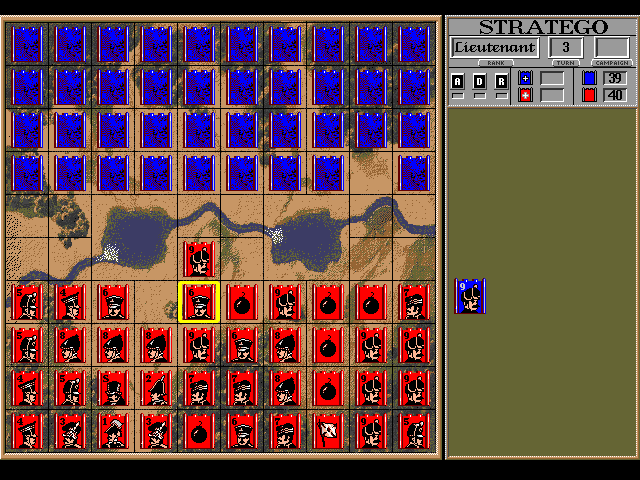
\includegraphics[width=0.7\textwidth]{figures/stratego.png}
    \caption{Stratego Game board.}
    \label{fig:stratego_review}
\end{figure}



\section{Board Games in Community Building}
Modern board games are becoming more widespread, expanding their market share each year. During COVID-19 lockdowns, board game sales increased because people were stuck at home with family and had free time. Also, playing board games during that time helped with stress, isolation, and anxiety. Certain games like Pandemic, a cooperative strategy board game where players work together to stop global disease outbreaks by discovering cures before time runs out, became more popular due to their reflection of the real-world scenario. Board game communities differ between the West and the East \cite{boardgamehk}. From the east, board games are considered social activities, while in the west, board games grew as hobbies, communities focusing on the gameplay and mechanics. In Hong Kong, there are two distinct board game communities named BGHK and Oasis. BGHK consists of Cantonese-speaking individuals who treat board games as social bonding. They even event sessions for "party game days" and "welcome newbies," emphasizing making friends rather than the game itself. While the Oasis group focuses on the hobby, playing newly released and complex games. Attracting players with the mechanics and novelty rather than just socializing. A study has been made to use board games as an answer to the problem of difficulty in creating a sense of "togetherness or kinship," and board games have advantages for improving the cognitive function of older people \cite{Boardgames}. In the study, the Tresna Werdha Budi Pertiwi Social Home has a problem of having a sense of family among residents. By playing together, the elderly had consistent interaction with each other, reducing the feeling of loneliness and detachment. Board games not only provide entertainment but also memory stimulation and improve social bonds. Board games provide a face-to-face interaction requiring people to sit together at a table, unlike in video games, where players are often separate from each other \cite{boardgamecom}. Every shared experience creates a unique microenvironment where players enter a separate reality governed by the game's rules. In the space, the players share emotions and strategy. Sharing these emotions helps strengthen friendships, family bonds, and trust. Many board game players first connect through gaming with friends and family, which can branch out to dedicated groups or conventions, and expand their social circle.

\section{Other Applications}
An extension of MARL with DQN was demonstrated in robotics. In these environments, robots are trained to make decisions based on rewards. The study assigned different energy costs to each robotic arm, allowing the robot to learn how to adjust its movement based on cost, using less energy when the reward is small and exerting more effort if the reward is appropriate \cite{robotmarl}. MARL with Deep Q-learning was also used in traffic signal control. Applied a cooperative multi-agent DQN framework to manage six interconnected intersections, where each intersection acted as an independent learning agent. Using the SUMO simulator, each agent selected signal phases to minimize congestion and improve overall traffic flow. Their approach introduced a reward function based on the standard deviation of stopping vehicles across lanes, showing balanced lane utilization rather than simply reducing queue lengths. This design showed that MARL with DQN can enhance not only traffic efficiency but also environmental sustainability by reducing emissions and fuel consumption. In businesses in developing countries, it is essential that growth should be the top priority; however, this creates a problem in increasing taxation for improving infrastructure to further support the current population. Using MARL, we can create a model system where multi-agent RL acts as different parties that discover the optimal tax policies without needing to rely on traditional economic models \cite{MARLEcon}.

\section{Application to Other Game Environments}
Although this study focuses on Stratego as the game environment, the MARQ framework can also be applied to other strategic and simulation-based games that involve decision-making and hidden information. Sports management titles such as Madden NFL's Dynasty Mode, NBA 2K's franchise mode, Esports Manager, and Football Manager feature complex systems of player development, transfer, and long-term planning, where agents must act without complete information about the future player performance and market behavior. In these environments, the MARQ framework could model AI agents capable of learning optimal trade strategies or budget allocations through reinforcement learning. The framework's belief-state modeling would allow the AI to check hidden player attributes or opponent strategies, while the Deep Q-Network could optimize sequential decisions across multiple simulated seasons.

Similarly, the framework could be applied to a game called Clash Royale, where players must make fast tactical decisions without full knowledge of their opponent's hand or resource level. The Probabilistic Belief State in this setting could estimate the likelihood of specific opponent cards being available, while the Deep Q-Network would select optimal actions for troop deployment and timing. IS-MCTS could be used to search over possible opponent hands, enabling informed decision-making for lane control or counter-attack scenarios.



\chapter{Theoretical Frameworks}

\section{Stratego Game Domain}

Stratego is an imperfect information board game with European roots, popularized in the Netherlands in the 1940s and released in North America in 1961 \cite{perolat2022stratego}. The game is played on a 10x10 board that includes two 2x2 ``lake'' areas in the center, which are impassable. Each player commands an army of 40 pieces of varying ranks, and during the game, the identity and rank of the pieces are kept secret from the opposing player. The objective is to capture the opponent's flag or eliminate all of their movable pieces.

Each army consists of 12 different types of pieces, with ranks ranging from 1 (the Spy) to 10 (the Marshal), alongside Bombs and a Flag. Higher-ranked pieces defeat lower-ranked ones during combat, except in special situations: the Spy can defeat a Marshal if attacking first, the Miner is the only piece that can defuse Bombs, and Scouts can move multiple squares in a straight line. There are 3 ways to win the game capturing the flag, immobilizing all movable enemy pieces, or forcing the opponent to run out of time.


\begin{figure}[ht]
    \centering
    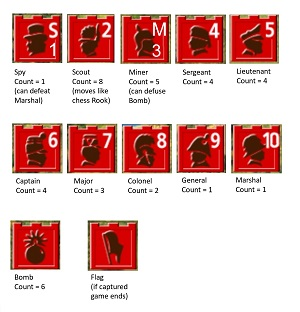
\includegraphics[width=0.5\textwidth]{figures/stratego_piece.png}
    \caption{Stratego pieces.}
\end{figure}

\begin{figure}[ht]
    \centering
    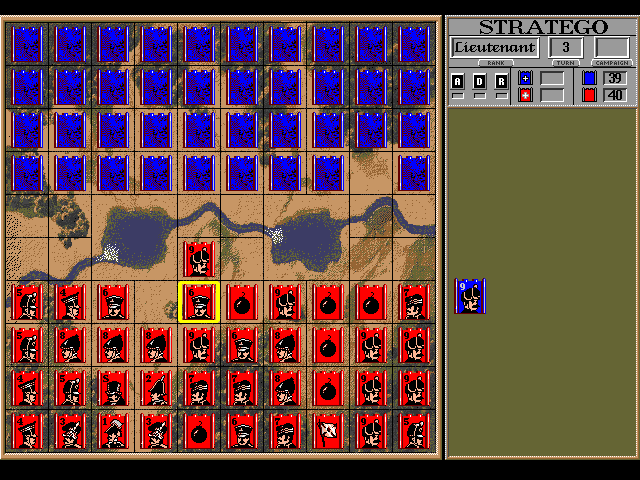
\includegraphics[width=0.7\textwidth]{figures/stratego.png}
    \caption{Stratego Game board.}
    \label{fig:stratego_tech}
\end{figure}

The high theoretical state space of Stratego shows how difficult the game is to solve:

\begin{equation}
|\mathcal{S}| = \binom{40}{1,1,2,3,4,4,4,5,8} \times 10^{10} \times 2^{40} \approx 10^{535}
\end{equation}

Perolat et al. \cite{perolat2022stratego} established the permutation for game state. The agent must use reasoning with limited information rather than trying to look at every possible outcome, making the computation intractable.


\section{MARQ Framework Overview}

The MARQ framework is a Multi-Agent Rainbow Deep Q-Networks system that trains agents through self-play and deep reinforcement learning \cite{AlphaStratego}. Agents learn by competing against many different opponents, including their own previous versions and exploratory variants, within a league-based self-play system.

The central problem is reasoning about hidden information without enumerating every possible state. The number of possible game states exceeds $10^{535}$, and initial setups reach $10^{66}$ per player \cite{perolat2022stratego}. MARQ handles this scale through implicit belief representations, probabilistic reasoning, and pattern recognition. Deep reinforcement learning estimates values. Attention mechanisms process game history. Mixed strategies prevent exploitation. The system keeps all of these computations fast enough to run in real time.

The architecture connects these components in a pipeline. The AAREN module takes raw game positions and move sequences, then produces learned embeddings that encode opponent piece identity inferences. These embeddings form the base for all subsequent reasoning. A league-based training method trains and evaluates MARQ agents simultaneously.



\begin{table}[htbp]
    \centering
    \caption{Key symbols and descriptions.}
    \label{tab:MARQ-symbols}
    \begin{tabular}{|l|p{4cm}|p{6cm}|}
        \hline
        \textbf{Symbol} & \textbf{Description} & \textbf{Example (MARQ Framework)} \\
        \hline
        $\pi_i(a|I_i)$ & Policy for agent i choosing action a given information set $I_i$ & Probability of moving a piece forward given current visible board state and belief about opponent pieces \\
        \hline
        $\mathcal{B}_t$ & Implicit belief representation at time t & Probability distribution over possible identities and positions of hidden opponent pieces inferred by AAREN \\
        \hline
        $v^{\pi}_i(h, \mathcal{B}_t)$ & Value function for agent i following policy $\pi$ given history h and belief $\mathcal{B}_t$ & Expected reward for current board position considering uncertainty about opponent setup \\
        \hline
        $Q_{\text{network}}(s', a)$ & Deep Q-Network approximation of action-value function & Neural network estimate of value for attacking with a suspected Marshal vs opponent piece \\
        \hline
        $R^{\text{capture}}{i,t+1}$ & Immediate reward from piece captures weighted by piece values & +9 points for capturing opponent Marshal, -1 for losing a Scout \\
        \hline
        $O = \{o_1, \dots, o_t\}$ & Observation sequence processed by AAREN attention mechanism & Sequence of board states, moves, and attack outcomes throughout the game \\
        \hline
        $\alpha_i$ & Attention weights for historical observations in AAREN & Higher weight on turn when opponent's Marshal was revealed, lower on routine Scout moves \\
        \hline
        $\pi^*$ & Nash equilibrium policy profile & Optimal mixed strategy that cannot be exploited by opponent strategy changes \\
        \hline
        $Q_{eval}(\mathcal{B})$ & Embedding quality evaluator output & Confidence score for learned representation accuracy \\
        \hline
        $H(\pi)$ & Policy entropy measure & Ensures minimum unpredictability to prevent exploitation \\
        \hline
        $\epsilon$ & Exploration rate for agent behavior & Controls exploration vs exploitation balance in multi-agent learning \\
        \hline
        $\gamma$ & Discount factor for future rewards & Importance of long-term vs immediate rewards in value estimation \\
        \hline
    \end{tabular}
\end{table}


\section{MARQ Policy Definition}

Policy optimization in reinforcement learning improves an agent's strategy to maximize total reward \cite{DRLImperfectInfo2023}. Games with hidden information and multiple players demand policies that perform well against fixed opponents while also handling uncertainty and shifting strategies from other agents. MARQ connects belief state reasoning with value-based decisions to meet these demands.

Policy learning in MARQ serves two goals. The first is winning games through tactical choices. The second is improving the quality of the embeddings that the AAREN module produces. The two objectives reinforce each other: better embeddings sharpen decision-making, and good decisions reveal opponent information that in turn refines the embeddings.

\subsection{Core Policy Framework}

A policy in the MARQ framework, denoted $\pi_i(a|I_i)$, defines a probability distribution over actions for agent $i$ conditioned on its current information set $I_i$. In perfect information games, policies operate on complete game states. MARQ policies do not have that luxury. They reason under uncertainty about the true state of the environment. The information set $I_i$ contains all observations available to the agent: visible board positions, revealed piece identities, and the history of observed movements and combat outcomes.

The core difficulty is that agents must act without knowing the opponent's private information. In Stratego, this means the rank and position of every unrevealed opponent piece remain unknown. The policy must incorporate estimates of the opponent's pieces into its decision process and select actions that perform well across many possible hidden states.

MARQ addresses this by using implicit belief representations $\mathcal{B}_t$ rather than enumerating every possible game state. The AAREN module learns and updates these representations as new information arrives. The policy takes the following form:

\begin{equation}
\pi_i(a|I_i, \mathcal{B}_t) = P(\text{action} = a \mid \text{information set } I_i, \text{implicit belief } \mathcal{B}_t)
\end{equation}

The policy learns to weight actions based on their expected value across the inferred distribution of opponent configurations rather than optimizing for a single specific setup. Playing well requires this kind of reasoning about hidden states.

\subsection{Implicit Representation Optimization}

The quality of the implicit belief representation directly affects decision quality. Inaccurate inferences produce poorly calibrated action values. MARQ therefore treats representation accuracy as an auxiliary training objective and uses revealed piece identities as supervised labels for embedding refinement.

When combat reveals the piece identities, the system calculates the prediction error using Kullback-Leibler (KL) divergence.

\begin{equation}
\mathcal{E}_{\text{pred}}(t) = \sum_{p \in \text{Pieces}_{\text{revealed}}(t)} D_{\text{KL}}\left(\text{Representation}_t(p) \| \delta_{s^*_p}\right)
\end{equation}

Here, $\delta_{s^*_p}$ denotes the Dirac delta distribution concentrated on the true piece type. The error quantifies how far the predicted distribution lies from the actual identity.

This prediction error becomes a representation accuracy reward signal. It encourages the policy to develop embeddings that better predict actual piece configurations:

\begin{equation}
R_{\text{accuracy}}(t) = -\mathcal{E}_{\text{pred}}(t) = -\sum_{p \in \text{Pieces}_{\text{revealed}}(t)} \left[\text{Representation}_t(p=s^*_p) > 0\right] \cdot \log \text{Representation}_t(p=s^*_p)
\end{equation}

The optimal policy maximizes the joint objective of game outcomes and representation accuracy:

\begin{equation}
\pi^*_i = \arg\max_{\pi_i} \mathbb{E}_{\tau \sim \pi_i}\left[\sum_{t=0}^T \gamma^t \left(R_{\text{game}}(t) + \eta \cdot R_{\text{accuracy}}(t)\right)\right]
\end{equation}

The hyperparameter $\eta \in \mathbb{R}^+$ controls the relative importance of representation accuracy versus immediate game rewards.

The value function in MARQ extends the standard Bellman equation to account for belief dynamics. It expresses the expected cumulative reward as a function of the current information set and implicit belief.

\begin{equation}
v^{\pi}_i(I, \mathcal{B}_t) = \mathbb{E}_{\pi}\left[R^{\text{capture}}_{i,t+1} + \lambda_1 R^{\text{info}}_{i,t+1} + \lambda_2 R^{\text{position}}_{i,t+1} + \gamma v^{\pi}_i(I_{t+1}, \mathcal{B}_{t+1}) \mid I_t = I, \mathcal{B}_t\right]
\end{equation}

Three strategic components make up the reward function. The capture reward $R^{\text{capture}}$ reflects material changes. The information reward $R^{\text{info}}$ quantifies the value of information revelation. The position reward $R^{\text{position}}$ measures territorial control.

MARQ training aims to reach a Nash equilibrium. At equilibrium, no player can improve their expected payoff through unilateral deviation. This stability ensures that the policy remains robust against adversarial exploitation.

\begin{equation}
v_i(\pi^*) = \max_{\pi_i} v_i(\pi_i, \pi^*_{-i})
\end{equation}

Finding exact Nash equilibria in large imperfect information games is computationally intractable. MARQ instead seeks approximate equilibria through self-play training with diverse opponent populations.


\section{Deep Q-Network Architecture}

The Deep Q-Networks in MARQ operate on implicit belief representations rather than complete game states \cite{DRLImperfectInfo2023}. The network approximates Q-values over probability distributions of opponent configurations, $\mathcal{B}_t$:
$$Q(s, a) = \mathbb{E}_{s' \sim \mathcal{S}_t \subseteq \mathcal{B}_t}[Q_{network}(s', a)]$$

A standard replay buffer stores experience. Transitions $(\mathcal{B}_t, a_t, r_t, \mathcal{B}_{t+1})$ are sampled uniformly to train the value function.

\subsection{Rainbow DQN Components}
The implementation incorporates several enhancements from the Rainbow DQN architecture \cite{RainbowJMLR2021} to improve stability and sample efficiency.

\paragraph{Distributional RL (Categorical DQN).}
Categorical DQN (C51) models the value distribution directly. It captures the inherent uncertainty of the game by approximating the distribution with 51 atoms spanning the range from $V_{min}$ to $V_{max}$.

\begin{equation}
Z_\theta(s, a) = \sum_{i=1}^{N} p_i(s, a) \delta_{z_i}
\end{equation}
Training minimizes the Kullback-Leibler divergence between the predicted distribution and the projected target distribution:
\begin{equation}
D_{KL}(\Phi \hat{\mathcal{T}} Z_{\theta'} || Z_\theta)
\end{equation}
where $\Phi$ is the projection operator that maps the Bellman update onto the fixed support atoms.

\paragraph{Noisy Networks for Exploration.}
Noisy Linear layers inject learned noise into the network weights. The agent maintains an unpredictable strategy without a separate exploration schedule, and the network itself optimizes the degree of exploration required for each state.

\begin{equation}
y = (\mu_w + \sigma_w \odot \epsilon_w)x + (\mu_b + \sigma_b \odot \epsilon_b)
\end{equation}

\paragraph{Dueling Network Architecture.}
The network separates state value estimation $V(s)$ from advantage estimation $A(s, a)$ using two streams that share a common convolutional feature extractor:
\begin{equation}
Q(s, a; \theta, \alpha, \beta) = V(s; \theta, \beta) + \left( A(s, a; \theta, \alpha) - \frac{1}{|\mathcal{A}|} \sum_{a'} A(s, a'; \theta, \alpha) \right)
\end{equation}
This decomposition improves policy evaluation when many actions carry similar value.

An exploration bonus augments the Q-values. The bonus is based on the uncertainty of the inferred representation, following an optimism-in-the-face-of-uncertainty approach.

\begin{equation}
Q_{augmented}(s, a) = Q_{base}(s, a) + \lambda \cdot U(a)
\end{equation}
Here $U(a)$ represents the entropy of the learned distribution at the target location. This term encourages the agent to investigate unknown opponent pieces.

\subsection{Training Stability via Regularization}

The Ataraxos system reached superhuman performance in no-press Diplomacy, and its designers found that training stability matters as much as the algorithm itself \cite{Ataraxos2025}. Deep reinforcement learning agents face two recurring problems: wasting updates on low-information experiences, and cycling between strategies without settling on a robust one.

\paragraph{Advantage Filtering for Sample Efficiency.}
Advantage filtering concentrates learning on the most informative transitions \cite{RegularizationStrategyExploration}. In reinforcement learning, the temporal-difference (TD) error measures the gap between predicted values and outcomes. A standard replay buffer samples past transitions at random, treating every move equally. Advantage filtering breaks this uniformity. It samples the buffer and retains only the transitions with the largest TD errors:
\begin{equation}
\mathcal{B}_{filtered} = \text{Top}_{n/k}\left(\mathcal{B}_{sampled}, |\delta_i|\right)
\end{equation}
where $\delta_i = r_i + \gamma^n V(s'_i) - V(s_i)$ is the $n$-step TD error for transition $i$.

\paragraph{Dynamic Damping with Power-Law Annealing.}
Strategy cycling is addressed through two regularization terms in the loss function, both based on Kullback-Leibler divergence:
\begin{equation}
\mathcal{L}_{total} = \mathcal{L}_{C51} + \alpha(t) \cdot D_{KL}(\pi \| \pi_{uniform}) + \beta(t) \cdot D_{KL}(\pi_{target} \| \pi)
\end{equation}

The coefficients follow power-law schedules with opposing dynamics:
\begin{align}
\alpha(t) &= \alpha_0 \cdot (1 - t/T)^p \\
\beta(t) &= \beta_0 + (\beta_T - \beta_0) \cdot (t/T)^p
\end{align}
where $t$ is the current episode, $T$ is the total training duration, and $p=2$ produces quadratic curves. Early in training, when uncertainty is highest, the agent explores aggressively. As the policy matures, the schedule shifts weight toward stability.


\section{AAREN and Learned Embedding System}

The AAREN module (Attention as Recurrent Neural Network) \cite{Aaren} serves as the memory and history system within MARQ. It does not maintain simple counts of piece identities. Instead, it produces learned embeddings from opponent moves, and the agent interprets these embeddings through training. AAREN handles long sequences in Stratego. It retains details over hundreds of moves while avoiding the gradient problems that degrade older models such as LSTMs. An attention mechanism lets AAREN look back across the full sequence of moves at once \cite{Aaren}.

\subsection{Recurrent Attention Computation}
AAREN implements an attention-based recurrent computation that maintains a state triplet $(a_t, c_t, m_t)$ across the observation sequence. Traditional recurrent neural networks suffer from vanishing gradients over long sequences. AAREN avoids this entirely. It provides direct access to the full history through attention weights while maintaining $O(1)$ inference complexity per timestep.

Given a sequence of observations $O = \{o_1, \ldots, o_t\}$ where each $o_i$ encapsulates the visible board state and public action outcomes, the AAREN cell first projects each observation into key and value representations:

\begin{equation}
k_t = W_k(o_t), \quad v_t = W_v(o_t)
\end{equation}

The projection matrices $W_k$ and $W_v$ are learned during training. The key $k_t$ determines how relevant the current observation is for belief updates. The value $v_t$ encodes the informational content to be integrated into the belief representation. The attention score $s_t$ measures the relevance of the current observation relative to a learned query vector $q$:

\begin{equation}
s_t = q^T k_t
\end{equation}

The weighted value accumulator $a_t$ aggregates value representations across the sequence:

\begin{equation}
a_t = a_{t-1} \exp(m_{t-1} - m_t) + v_t \exp(s_t - m_t)
\end{equation}

The term $\exp(m_{t-1} - m_t)$ rescales the previous accumulator when a new maximum appears. The term $\exp(s_t - m_t)$ computes the relative attention weight for the current observation. The normalization constant $c_t = c_{t-1} \exp(m_{t-1} - m_t) + \exp(s_t - m_t)$ ensures that the effective attention weights sum to unity. The output $h_t = a_t / c_t$ is an attention-weighted aggregation of all observations up to time $t$.

\subsection{Piece Type Inference}
AAREN infers piece types from action sequences. Each action is encoded as a 24-dimensional feature vector capturing movement patterns, contextual information, and game state features. The network outputs a probability distribution over piece types:

\begin{equation}
P(\text{piece\_type} = t \mid \text{action\_sequence}) = \text{softmax}(W_{out} \cdot h_T + b_{out})_t
\end{equation}

The network combines these embeddings with game rules and the board state to improve decisions under uncertainty.

An evaluation system monitors embedding quality and drives improvement. A neural network evaluator takes embeddings as input and outputs quality scores $Q_{eval}(\mathcal{E}) = \text{MLP}(\mathcal{E}; \theta_{eval})$. Training compares predictions against true piece identities:

\begin{equation}
R_{quality}(\mathcal{B}, g) = \alpha \cdot \mathcal{B}[g] - \beta \cdot |V_{pred} - V_{actual}| - \gamma \cdot \text{distance\_penalty}
\end{equation}

The system decides when additional information gathering is worth the cost through uncertainty assessment:

\begin{equation}
\text{NeedMoreInfo}(\mathcal{B}) = \mathbb{1}\{H(\mathcal{B}) > \theta_H\} \cdot \mathbb{1}\{Q_{eval}(\mathcal{B}) < \theta_Q\}
\end{equation}

\subsection{Embedding Updates on Piece Revelation}

When a battle reveals a piece's true type, the AAREN embeddings synchronize with ground truth. The inferred distribution at the revealed position collapses to certainty:
\begin{equation}
\text{Representation}_{pos}[t] = \begin{cases}
1.0 & \text{if } t = g \\
0.0 & \text{otherwise}
\end{cases}
\end{equation}

The system increments the revealed piece count and adjusts remaining beliefs to respect piece count constraints. For unrevealed positions $p \neq pos$:
\begin{equation}
\mathcal{B}_p[t] \leftarrow \mathcal{B}_p[t] \cdot \frac{\text{max\_count}[t] - \text{revealed\_count}[t]}{\text{remaining\_count}[t]}
\end{equation}

For example, when the single Marshal is revealed, the probability of any other piece being a Marshal drops to zero.

\subsection{Hindsight-Aided Belief Refinement}

The AAREN module provides inference during gameplay. The Hindsight-Aided Belief Refinement (HABR) module adds a second channel: learning from verified information. When combat reveals a piece, HABR applies retrospective learning across the entire history of that piece, using the ground truth as a supervisory signal for past predictions.

\paragraph{Information Gain Reward.}
The Information Gain reward quantifies how much an observation reduces uncertainty about opponent pieces. Let $H(P)$ denote the Shannon entropy of a probability distribution $P$. The KL divergence from a uniform prior $U$ over $N$ piece types is:
\begin{equation}
D_{KL}(P \parallel U) = \log(N) - H(P)
\end{equation}
The Information Gain reward measures the change in this divergence between consecutive representation updates:
\begin{equation}
R_{gain}(t) = D_{KL}(\text{Rep}_{t-1} \parallel U) - D_{KL}(\text{Rep}_t \parallel U)
\end{equation}
Substituting the divergence formula yields:
\begin{equation}
R_{gain}(t) = (\log(N) - H(\text{Rep}_{t-1})) - (\log(N) - H(\text{Rep}_t)) = H(\text{Rep}_{t-1}) - H(\text{Rep}_t)
\end{equation}
$R_{gain}$ equals the reduction in entropy. A positive reward occurs only when the observation at time $t$ increases certainty about piece identity relative to $t-1$. This aligns the agent's incentives with active information gathering.

\paragraph{Sinkhorn Constraint Normalization.}
Independent belief updates for each piece position can produce inconsistent global predictions. Without piece count constraints, the model might assign high probability to multiple pieces being the single Marshal. This phenomenon is called identity inflation. It violates the physical constraints of the game.

Sinkhorn normalization corrects this through iterative proportional fitting. Given a representation matrix $M \in \mathbb{R}^{P \times S}$ where $P$ is the number of tracked pieces and $S$ is the number of piece types, two constraints must hold. The row constraint $\sum_{s} \text{Rep}(p, s) = 1$ ensures each piece has exactly one identity. The column constraint $\sum_{p} \text{Rep}(p, s) = Count(s)$ ensures the total predicted count of each piece type matches the remaining count.

The Sinkhorn algorithm alternates between row and column normalization until convergence. The approach is differentiable, so gradients pass through it. When piece A is confirmed as the Spy, the Sinkhorn layer automatically redistributes probability across all other pieces, creating a shared update across the entire inferred state.


\section{Multi-Agent Learning and Strategy Mixing}

\subsection{League-Based Training Architecture}
The league maintains a changing pool of agents so that the model encounters many different strategies \cite{perolat2022stratego}. The main agent is the best current policy under training. The historical pool stores earlier versions of the main agent, each representing a different stage of development.

Opponents are sampled during training according to a fixed probability distribution.
\begin{equation}
P(\text{opponent}) = 
\begin{cases} 
0.5 & \text{Main Agent (Self-Play)} \\
0.5 & \text{Uniform}(\text{Historical Pool})
\end{cases}
\end{equation}
This prevents the agent from cycling through the same strategies repeatedly. It must defeat all previous versions of itself.

\subsection{Strategy Mixing for Exploitation Resistance}

Deterministic strategies in extensive-form imperfect information games are inherently suboptimal \cite{perolat2022stratego, MARLGametheoretic}. An adversary who knows a deterministic policy reduces the game to a perfect information setting, eliminating the strategic uncertainty that defines games like Stratego. MARQ counters this through two complementary mechanisms.

At the action selection level, Noisy Linear layers inject learned, state-dependent noise into the policy. The network learns the appropriate degree of randomization for each game state rather than relying on fixed exploration schedules such as $\epsilon$-greedy.

At the strategy level, diverse opponent exposure during training achieves mixing. The league system maintains a population of historical agent checkpoints, each representing a different strategic approach discovered during training. Action randomness combined with strategy variety produces policies that are unpredictable and resistant to exploitation.

\subsection{Multi-Dimensional Reward Structure}

The reward function $R(s, a, s')$ guides learning in Stratego's sparse-reward environment \cite{PBRSModern2022}:

\begin{equation}
R_{total} = R_{move} + R_{capture} + R_{tactical} + R_{info}
\end{equation}

The move reward $R_{move}$ gives small bonuses for advancing pieces (approximately $+0.05$) to encourage active play. The capture reward $R_{capture}$ scales by the rank of the captured piece according to $0.15 \times \frac{\text{Rank}}{11.0}$. The tactical reward $R_{tactical}$ assigns specific bonuses for key strategic captures: $+0.5$ for Miner vs Bomb defusals and $+1.0$ for Spy vs Marshal assassinations. The information reward $R_{info}$ provides $+0.3$ for revealing high-value opponent pieces.

The framework uses \textit{Reward Annealing} to transition from tactical learning to strategic gameplay. Dense shaping rewards are scaled down as the training curriculum advances. In later training phases, these auxiliary signals are completely removed, and the agent relies exclusively on sparse, terminal win/loss rewards. This progression prevents the agent from developing sub-optimal behaviors driven by short-term shaping incentives.


\section{Specialized Agent Architectures}

\subsection{Setup Agent via Distributional RL}

A specialized SetupAgent handles the game's initial setup. It learns optimal piece configurations by treating the placement phase as a sequential decision process. The state representation is a 3-channel input tensor: one channel encodes the current board state with already-placed pieces, a second provides a valid positions mask indicating legal placement locations, and a third identifies which piece type is currently being placed.

The agent outputs a distributional Q-value for each of the 100 board positions, mapping $Q(s, pos)$ to a distribution over $[V_{min}, V_{max}]$. This distributional approach captures the inherent uncertainty in setup quality, since the true value of a placement depends on the unknown opponent configuration.

An exploitability critic network penalizes predictable placements to prevent static, easily countered setups:

\begin{equation}
\mathcal{L}_{total} = \mathcal{L}_{C51} + \lambda \cdot \mathcal{L}_{predictability}
\end{equation}


\subsection{Information Set Monte Carlo Tree Search (IS-MCTS)}

For high-stakes decisions, especially in the endgame, MARQ uses an Information Set MCTS agent \cite{UpdatedISMCTS} that combines search with learned value functions. The search operates in three phases.

In the determinization phase, the agent samples a consistent concrete world state $s_{det}$ from the history-based beliefs according to $s_{det} \sim P(S | \mathcal{B}_t)$. This converts the imperfect information game into a perfect information instance for the duration of the simulation.

In the tree traversal phase, a UCB1 variant navigates the search tree to balance exploration and exploitation of move sequences. Nodes represent information sets rather than individual states, so the tree can be shared across multiple determinizations.

In the leaf evaluation phase, terminal or unexpanded nodes are evaluated using the Rainbow DQN value function instead of random rollouts:

\begin{equation}
V(s_{leaf}) \approx Q_{DRQN}(s_{leaf}, a_{best})
\end{equation}


\section{Game Environment and State Management}

The Stratego environment provides the foundation for agent training and evaluation. It manages the complex dynamics of imperfect information.

\subsection{Information Set Management}
The environment maintains distinct representations for each information context:

\begin{equation}
\mathcal{I}_{player} = \{s : s \text{ is consistent with player observations}\}
\end{equation}

Each player receives only the subset of game state information available through its observation function.

\subsection{Temporal State Evolution}
Game states evolve according to an update function.

\begin{equation}
s_{t+1} = \text{EnvStep}(s_t, a_t^1, a_t^2, \theta_t)
\end{equation}

Here $\theta_t$ represents stochastic elements such as hidden information revelation and time limits.

\subsection{Valid Action Filtering}
The environment enforces game rules through valid action constraints:

\begin{equation}
\mathcal{A}_{valid}(s, player) = \{a : \text{IsLegalMove}(a, s, player) \land \text{RespectsGameRules}(a, s)\}
\end{equation}

Only legal moves consistent with Stratego's rules and piece capabilities are available to the agent.

\subsection{Piece Setup and Initialization}
Setup policies govern strategic piece placement.

\begin{equation}
\pi_{setup}(\text{placement}|player) = \text{NeuralNetworkSetup}(\text{strategic\_features}, \theta_{setup})
\end{equation}

Strategic features include positional value maps, piece interaction potentials, and defensive vulnerabilities. The initial placement of pieces is a high-impact decision that shapes the remainder of the game \cite{PlacementSetup}.

\section{MARQ Move Selection and Decision-Making}

The MARQ framework's architectural components converge in the real-time move selection process. Algorithm \ref{alg:marq_decision} details this procedure, which integrates learned positional priors with tactical search to optimize behavior in adversarial environments.

\begin{algorithm}
\caption{MARQ: Decision-making and Move Selection}
\begin{algorithmic}[1]
\REQUIRE Public Observations $O$, Board State $S$, DQN weights $\theta$, AAREN weights $\phi$, Temperature $T$
\ENSURE Optimal Action $a^*$
\STATE $\mathcal{H}_t \gets \text{UpdateAggregation}(O, \phi)$ 
\STATE $\mathcal{B}_t \gets \text{GetSoftmaxBeliefs}(\mathcal{H}_t)$ 
\STATE $X_t \gets \text{Concatenate}(S, \mathcal{H}_t)$ 
\STATE $Q(s, \cdot) \gets \text{RainbowInference}(X_t, \theta)$ 
\STATE $\mathcal{A} \gets \text{LegalMoves}(S)$
\FORALL{$a_i \in \mathcal{A}$}
    \IF{$\text{IsAttack}(a_i, S)$}
        \STATE $target\_pos \gets \text{TargetSquare}(a_i)$
        \STATE $P \gets \mathcal{B}_t(target\_pos)$ 
        \STATE $V_{exp} \gets \sum_{r \in \mathcal{R}} P(r) \cdot \mathbb{U}(\text{Attacker}, r)$ 
        \STATE $V_{final}(a_i) \gets \lambda Q(s, a_i) + (1-\lambda) V_{exp}$
    \ELSE
        \STATE $V_{final}(a_i) \gets Q(s, a_i)$
    \ENDIF
\ENDFOR
\IF{Training/Self-Play and $T > 0$}
    \STATE $\pi(a_i) \gets \frac{\exp(V_{final}(a_i) / T)}{\sum_{a \in \mathcal{A}} \exp(V_{final}(a) / T)}$
    \STATE \textbf{return} $a^* \sim \pi(\cdot)$
\ELSE
    \STATE \textbf{return} $a^* \gets \arg\max_{a_i \in \mathcal{A}} V_{final}(a_i)$
\ENDIF
\end{algorithmic}
\label{alg:marq_decision}
\end{algorithm}

\subsection{Historical Context Update}
The decision process begins with the AAREN module's recurrent attention system. As game observations arrive, the history aggregator updates its internal state. The agent's current embedding thus reflects the opponent's cumulative behavioral patterns, not just the immediate board state.

\subsection{Probabilistic Belief Extraction}
After updating the history, the system extracts softmax probability distributions for hidden pieces. These piece-identity predictions are generated for every square on the board. They represent the agent's current belief about the hidden ranks of unrevealed opponent pieces.

\subsection{Information Set Tensorization}
The visible board state and the learned AAREN embeddings are concatenated to form a high-dimensional information set representation. In the current implementation, this produces a 79-channel input tensor (15 physical board features + 64 history embedding channels), which encapsulates both the physical layout and the inferred hidden context.

\subsection{Value Distribution Estimation}
The Rainbow DQN's convolutional backbone and C51 distributional head process the 79-channel tensor. This step estimates the $Q$-value distribution over 51 atoms for all possible actions. The distribution captures the multi-modal uncertainty inherent in the state.

\subsection{Action-Space Filtering}
Legal move masking ensures rule compliance and efficiency. The Q-network's output is filtered against the set of valid moves $\mathcal{A}$ defined by Stratego's rules. Illegal actions cannot be selected.

\subsection{Expectamax Search and Tactical Summation}
Standard adversarial search algorithms like Minimax assume an opponent who plays optimally to minimize the agent's utility. Many environments involve stochastic elements or hidden information that are better modeled as probabilistic transitions \cite{DRLImperfectInfo2023, SubgameSolving2021}. Algorithms addressing this class of problems introduce ``Chance Nodes'' into the game tree.

In Stratego, the identity of an opponent piece encountered during an attack is a stochastic variable. The Expectamax value is an exact summation over the rank probabilities provided by the belief extractor: 
\begin{equation}
\mathbb{E}[V] = \sum_{r \in \mathcal{R}} P(\text{target is rank } r) \cdot \mathbb{U}(\text{outcome vs } r)
\end{equation}
The agent can pursue tactical aggression when the probability of a successful capture outweighs the risk of piece loss. The decision is grounded in the AAREN's inference history.

\subsection{Stochastic Action Selection (Temperature Scaling)}
Rigid, exploitable behavior loops must be avoided during self-play and evaluation. The final action selection step uses Temperature Scaling (Boltzmann Options). Instead of choosing the action with the highest expected value via a hard \textit{argmax}, the agent samples from a stochastic softmax distribution parameterized by a temperature variable $T$. The probability of selecting action $a_i$ follows the Boltzmann distribution over the action values $V_{final}$:
\begin{equation}
\pi(a_i) = \frac{\exp\left(V_{final}(a_i) / T\right)}{\sum_{a \in \mathcal{A}} \exp\left(V_{final}(a) / T\right)}
\end{equation}
As $T$ approaches zero, the selection becomes deterministically greedy. When $T$ increases, near-optimal actions receive proportionally higher selection probabilities, injecting controlled variance. This stochasticity serves two purposes: it generates a diverse and unpredictable curriculum roster during league training, and it prevents tactical stagnation within recurring positional maneuvers.

\section{Generalizability}

The MARQ framework provides mathematical stability in adversarial settings and applicability to real-world domains beyond gaming. This section presents the convergence guarantees of the training methodology and the potential for transferring learned representations to non-gaming environments.

\subsection{Mathematical Convergence Properties}
MARQ provides theoretical guarantees for convergence and performance under specific conditions.

\subsubsection{Incremental Learning Bounds}
The algorithm bounds value function estimation error as follows:
\begin{equation}
\|V_t - V^*\|_\infty \leq \frac{C}{\sqrt{t}} + \epsilon_{approx}
\end{equation}
where $C$ depends on reward bounds and the discount factor, and $\epsilon_{approx}$ represents function approximation error.

\subsubsection{Implicit Representation Accuracy Bounds}
Representation accuracy improves with additional observations:
\begin{equation}
\mathbb{E}[\text{Accuracy}(\mathcal{B}_t)] \geq 1 - \exp(-\alpha \cdot N_{obs}(t))
\end{equation}
where $N_{obs}(t)$ is the cumulative number of informative observations and $\alpha$ is a positive constant.

\subsubsection{Strategy Convergence in Self-Play}
The league training methodology converges to $\epsilon$-Nash equilibria under standard monotonic improvement assumptions:
\begin{equation}
\lim_{T \to \infty} \| \pi_T - \pi^* \| \leq \epsilon
\end{equation}
for some $\epsilon > 0$ depending on the exploration parameters and opponent diversity. Hierarchical best-response maintenance, main-pool promotion thresholds, and diversity-driven exploration drive this convergence.

\subsection{Applied Generalizability}
The MARQ framework was developed for Stratego, but its architecture applies to broader problems involving partial observability and adversarial decision-making.

\subsubsection{Inference in Degraded Environments}
The occlusion-based curriculum combined with AAREN history aggregation provides a method for training agents to operate in degraded environments. In autonomous drone applications, sensors may fail or be obstructed by smoke or weather. MARQ's ability to maintain an implicit belief state allows continued navigation and objective completion despite sensor loss.

\subsubsection{Signal Intelligence and Pattern Discovery}
In adversarial signal environments such as electronic warfare, implicit representation learning can discover latent identities in high-dimensional signal data. The network treats signal history as an action sequence and learns to categorize threats without explicit labeling of every transmission.

\subsubsection{Industrial Automation and Predictive Maintenance}
MARQ's architecture can integrate sparse sensor readings over time to predict hidden anomalies or maintenance needs in complex manufacturing pipelines. This enables proactive adjustments before system failure occurs.

These convergence properties and the transferability of the learned embeddings support confidence in the framework's ability to handle high-stakes gameplay and transition to practical applications.

%\section{AI Transparency, Inclusion, and Originality of Intent}

%The development of the MARQ framework for Stratego was governed by intentionality and human-led architectural design. While large language models and generative AI have become ubiquitous in modern software development, their role in this research was strictly limited to tasks such as grammatical refinement, high-level brainstorming, and code debugging for modules and networking. Every core component of the MARQ system, including the AAREN history aggregator and the ResNet-based policy heads, was researched, evaluated, and implemented with the intent of mastering imperfect information games in the Stratego domain.

\section{Algorithmic Evolution and Architecture Ablations}

The final MARQ architecture emerged from systematic experimentation and the refinement of several reinforcement learning components. Multiple established algorithms were evaluated and replaced because of performance bottlenecks or insufficient strategic depth in the Stratego domain.

\paragraph{Value Optimization and Exploration.} 
Early iterations used a normal DQN with $\epsilon$-greedy exploration. This approach proved inadequate for Stratego's sparse rewards and led to early stagnation. The implementation was upgraded to a Rainbow DQN architecture incorporating Noisy Networks for state-dependent exploration. The standard double-DQN configuration was then replaced with a Dueling Head architecture, which improved value estimation accuracy in states where multiple actions carry similar utility. To mitigate overfitting to deterministic opponent policies during self-play, the system also employs \textit{Boltzmann Exploration} (Temperature Scaling). The opponent's action selection uses a temperature-scaled softmax over Q-values, injecting controlled stochasticity to produce a more robust training curriculum.

\paragraph{History and Memory Representation.} 
Initial attempts to manage hidden information relied on explicit Probabilistic Belief States. These states introduced prohibitive computational complexity and memory overhead. They required $O(N^2)$ updates that throttled training throughput. The framework moved to an implicit belief system powered by the AAREN architecture. Long Short-Term Memory cells for trajectory embeddings were also replaced by AAREN's attention-based recurrence, which provided more stable gradient flow over long sequences and better handled the non-Markovian nature of piece identity inference.

\paragraph{Architectural Refinements.} 
The convolutional backbone underwent several iterations, moving from standard deep convolutional stacks to a dedicated ResNet architecture. Testing identified 6 Residual Blocks as the optimal depth. This configuration provides full receptive field coverage of the 10x10 board while maintaining low inference latency. The optimizer was transitioned from standard ADAM to ADAMW to improve weight decay and policy loss stability.

\paragraph{Strategic Initialization and Efficiency.} 
The piece placement phase was initially modeled using an agentic SetupAgent trained through distributional reinforcement learning. This approach introduced exploitability risks and operational overhead. The project transitioned to a non-agentic, fixed Heuristic Setup Agent with randomized flag positioning. The change resolved the exploitability concern and provided substantial computational savings. The agentic setup required approximately 2 seconds per episode; the heuristic method completes in under 100 milliseconds. This optimization effectively halved the total training compute requirement.

\chapter{Methodology}
This chapter outlines the methodology employed to evaluate the effectiveness of an AI system based on MARQ in solving mind sports with imperfect information. The approach involves the development of a competitive system, followed by the evaluation of its performance through win-rate analysis against human players and an assessment of its adaptability across diverse game environments. The subsequent sections detail the processes and methods that will be used to achieve these research objectives.

\section{Project Planning}
This research will be conducted according to a structured plan encompassing participant selection, sample size determination, and experimental procedures. The project will follow a rapid prototyping approach for the design and implementation of the AI system. The timeline is segmented into four distinct phases. The development phase will run from September 2025 to February 2026, beginning with game environment development from September through November 2025, followed by AI training from December 2025 to January 2026, and concluding with system deployment in February 2026. The user testing phase will take place in March 2026, involving one-on-one matches and data collection activities. The final analysis and documentation phase will commence in April 2026, focusing on data analysis and manuscript preparation.

\subsection{Community Introduction to Stratego}
The introduction of the game Stratego to the participant community is a prerequisite for this study. This necessity arises from a complete lack of available local participants possessing prior knowledge of the game's rules or strategies. Unlike more popular games like Chess, Stratego's niche status means a pre-existing pool of experienced players is not available for participation to test against MARQ. Therefore, a structured introduction is essential to cultivate the necessary participant cohort from the ground up. This approach ensures all participants begin with a uniform baseline understanding. It allows for the parallel development of both human expertise and artificial intelligence, creating a synchronized learning environment where the adaptive capabilities of the MARQ system can be fairly assessed against a human cohort that is also in the process of learning.

\subsection{Participant Selection}
The participant selection process is designed to recruit a cohort of 20 individuals via convenience sampling, taking into account the project's resource constraints while still yielding a enough sample. The target demographic is enthusiasts of strategic mind sports of a diverse age and game experience.

Prospective participants will be screened to evaluate two key attributes. Their strategic game experience is key to ensuring a baseline aptitude, and second, their confirmed lack of prior knowledge of Stratego to ensure the study's "synchronized learning" premise. Ultimately, only those who successfully finish the screening phase will be admitted, guaranteeing they possess the necessary foundational skills to provide meaningful interaction with the MARQ system and substantive feedback.

\subsection{Experimental Procedures}
One-on-one matches between human participants and the MARQ system will be conducted on-site using a single device. To ensure consistency, each participant will receive a checklist outlining the procedures for interacting with the game.

Each session will last one (1) hour, during which participants must complete at least two (2) games against MARQ. Additional games may be played if the time permits. The following game statistics will be recorded will include the winner, total game duration, total moves per player, and the number and type of remaining pieces for both players. Immediately following the session, each participant will be given an evaluation form to provide open-ended feedback on their experience.

\section{System Development}
The system development consists of two components which is the game environment and MARQ. The game environment will be developed to serve as the interface for human players and the world in which the AI agent operates. While MARQ is the trained model to be used as the bot playing against the player.

\subsection{Piece Value Computation}
To inform MARQ's reward function and internal heuristics, a quantitative value was assigned to each piece in Stratego. This was achieved through a systematic process to account for the relative power of each piece.
\begin{enumerate}
\item {Initial Unweighted Calculation:} The value of each piece was first computed using the formula:
\[
\text{Unweighted Piece Value} = a - b
\]

where a is the number of pieces it defeats and b is the number of pieces it loses to.
\item {Normalization:} The computed values were then normalized to a range of [0,1] using min-max scaling to create a standardized set of weights, typically used in chess evaluation.
\item {Final Weighted Calculation:} The final value was then recomputed by weighting each interaction:
\[
\text{Final Piece Value} = \sum_{i \in \text{beats}} w_i \;-\; \sum_{j \in \text{loses to}} w_j
\]
\end{enumerate}
 
where \(w_i\) and where \(w_j\) are the normalized values of the pieces it beats or loses to, respectively. This provides a more accurate reflection of each piece's strategic importance.

\subsection{Handling Imperfect Information: Probabilistic Belief State (PBS)}
A key challenge in Stratego is the unknown identity of opponent pieces. To address this, the MARQ system will incorporate a Probabilistic Belief State (PBS). The PBS is a matrix that maintains a probability distribution for the identity of each of the opponent's unrevealed pieces. This belief state is updated throughout the game using two forms of reasoning:
\begin{itemize}
\item {Deductive Reasoning:} When a piece interaction occurs, the PBS is updated with absolute certainty. The probabilities of the unknown piece being a Scout, Miner, or Sergeant would be set to 0, and the remaining probabilities are renormalized.
\item {Inductive Reasoning:} The system infers piece identity from an opponent's behavior. For example, a piece that moves frequently and far is more likely to be a Scout. A piece that moves away from a threat exhibits defensive behavior, slightly increasing the probability that it is a high-value piece like the Flag or Marshal. These behavioral heuristics, based on aggression, defensiveness, and movement patterns, are used to adjust the probabilities in the PBS via Bayesian updates.

\item {Real state vs. PBS comparison:} The system compares the  PBS with the real state of the board and can be updated to allign more to the true piece for training. Training will have two stages separated, creating the belief state and later on normalizing the values from the real state to the PBS for a more accurate prediction. The main purpose of the PBS is to create a pseudo-perfect information game out of the imperfect information.
\end{itemize}

\section{Model Training}
The most time-intensive part of the research. Mainly due to the computation needed by the model to learn both exploration and exploitation. Since we are using a DQN model, the epsilon value in the first few games will be large, making the model have a higher likelihood of choosing random moves to try and explore. Once the epsilon value becomes smaller and smaller the model tends to follow what it thinks will be the optimal move.

The state representation provided to the DQN is crucial. It will be a multi-channel tensor including: (1) the location of the player's pieces, (2) the location of known opponent pieces, and (3) the complete Probabilistic Belief State (PBS) for all unknown pieces. 

Every 100 episodes, the target model or history model will be synced from the policy network, along with the memory replay by the AAREN.

\begin{figure}[htbp]
\centering
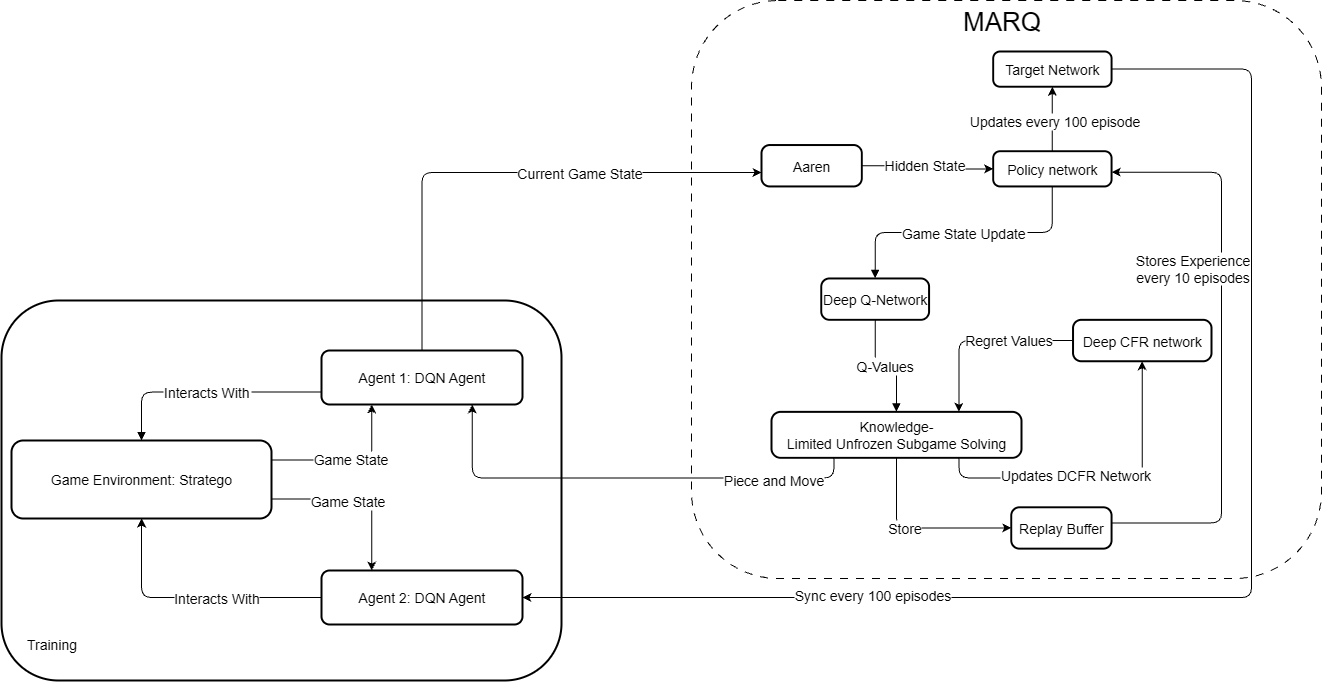
\includegraphics[width=1\textwidth]{figures/DQN Architecture.png}
\caption[MARQ Framework]{The MARQ System Architecture, which takes the Board State and PBS as input.}
\label{fig:my_label}
\end{figure}


\subsection{Deployment}
Upon completion of the training and validation cycles, the best-performing MARQ model weights will be saved and finalized for deployment. Deploy the trained model into the Stratego game environment described in Section 2 of the methodology.

The deployed system will function as the complete application used during the user testing phase. It will be configured to run locally on the single device designated for the experimental procedures. In this production mode, the model's exploratory functions will be deactivated for a more measured approach from the agent, always selecting the action with the highest predicted Q-value. This ensures that all human participants compete against the identical, optimized version of the MARQ AI, providing a consistent baseline for the quantitative and qualitative evaluations.

\begin{figure}[ht]
    \centering
    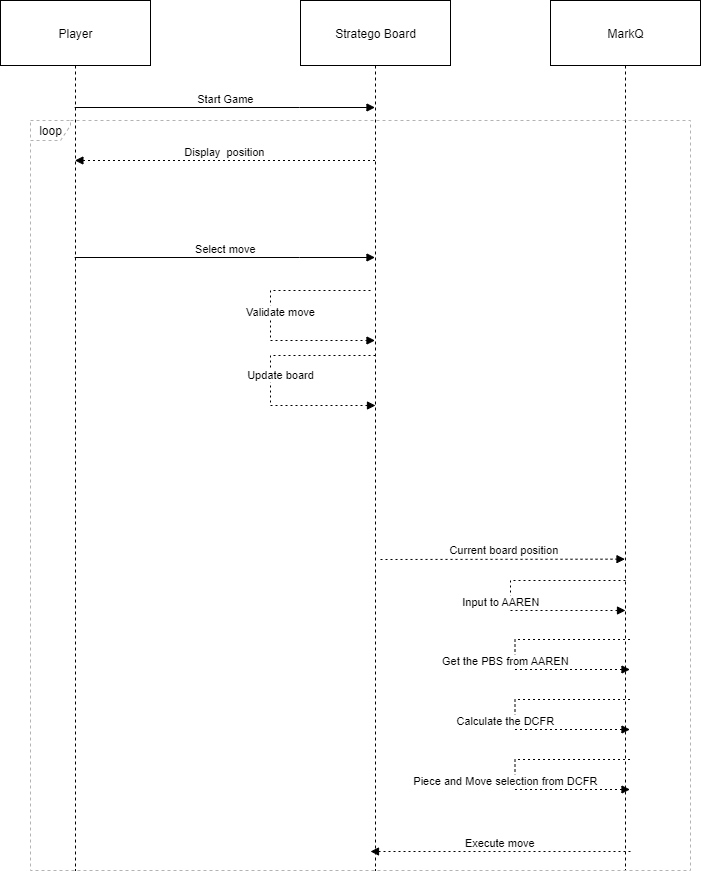
\includegraphics[width=.5\textwidth]{figures/Game diagram.png}
    \caption{Game Sequence Diagram}
    \label{fig:Sequence Diagram}
\end{figure}

In the figure above, the player starts the game and the loop begins until either the player wins by getting the flag of the agent or loses if the agent reaches the player's flag. The agent gets the current position and sends it to AAREN, constructing the possible positions of the board. After getting the PBS, it is then used to calculate the possible moves and actions that can be taken by the DeepCFR. Once the DeepCFR calculates pieces that are possible to have moves, it is then the role of the DQN to formalize a strategy to be used. 
\section{Evaluation}
A comprehensive evaluation approach combining quantitative and qualitative methods will be used to assess the MARQ system's performance and the user experience.

\subsection{Quantitative Analysis}
The quantitative assessment of the model's performance is conducted through the Evaluation component. Key metrics are tracked to gauge learning progress and strategic capability. Primary analytics include:
\begin{itemize}
\item {Win Rate\%}: The percentage of games won against human participants.
\item {Average Game Length}: The mean number of moves or duration of games, indicating game efficiency.
\item {Decision-Making Speed}: The average time taken by the agent to select an action.
\item {Loss Curves}: The progression of policy and value loss over training time, indicating the stability of the learning process.
\item {Player Performance over Time}: To evaluate the "synchronized learning" environment, a two-tailed paired t-test will be used. This will determine if there is a statistically significant difference in gameplay metrics (e.g., difference in remaining pieces) between a player's first and last games, assessing if human players improve against the AI.

The results from the Likert-scale questions will be analyzed using a weighted mean to derive a quantitative score for each dimension of user acceptance.
\end{itemize}

\subsection{Qualitative Analysis}
To assess the end-user opinion on usability, a usability testing session will focus on gathering participant feedback through an evaluation form. The form will evaluate three key dimensions:
\begin{itemize}
\item {Performance:} Assessing the agent's speed, consistency, and perceived strategic competence.
\item {Usability:} Evaluating the ease of use, intuitiveness of the interface, and overall user experience.
\item {Relevance:} Gauging the AI's value as a strategic tool and its potential for helping players learn Stratego.
\end{itemize}


\subsection{Model Version History}
The development of MARQ is an iterative process. Each model version represents a snapshot of this evolution, performance metrics, and reliability. 

\subsection{Initial Training}

Under Appendix B are the initial training results of 1000 training cycles or episodes. We can see that the early training phase is not yet refined due to the agent being in the exploratory phase, ready to search and find an exploitable strategy. The reward indicates that it is having a hard time finding a good strategy to fight against the other agent. The win-rate stayed to a draw due to the agents being on an endless loop of moving pieces back in forth. Another issue is that the agent has reduced epsilon, making the moves deterministic, and only picking the "best move" with the highest q-value. 

%%%%%%%%%%%%%%%%%%%%%%%%%%%%%%%%%%%%%%%%%%%%%%%%%%%%%%%%%%%%%%%%%%%%%%%%%%%
\chapter{Results and Discussion}
%%%%%%%%%%%%%%%%%%%%%%%%%%%%%%%%%%%%%%%%%%%%%%%%%%%%%%%%%%%%%%%%%%%%%%%%%%%

This chapter presents the training results and performance evaluation of the MARQ framework across different phases of the curriculum. The evaluation focus is on the agent's ability to acquire tactical knowledge and manage imperfect information.

\section{Training Progress and Convergence}

Training was conducted over 34,000 episodes, following the five-phase curriculum. Figure \ref{fig:training_progress} illustrates the convergence behavior of the Rainbow DQN agent.

\begin{figure}[htbp]
    \centering
    \begin{subfigure}[b]{0.48\textwidth}
        \centering
        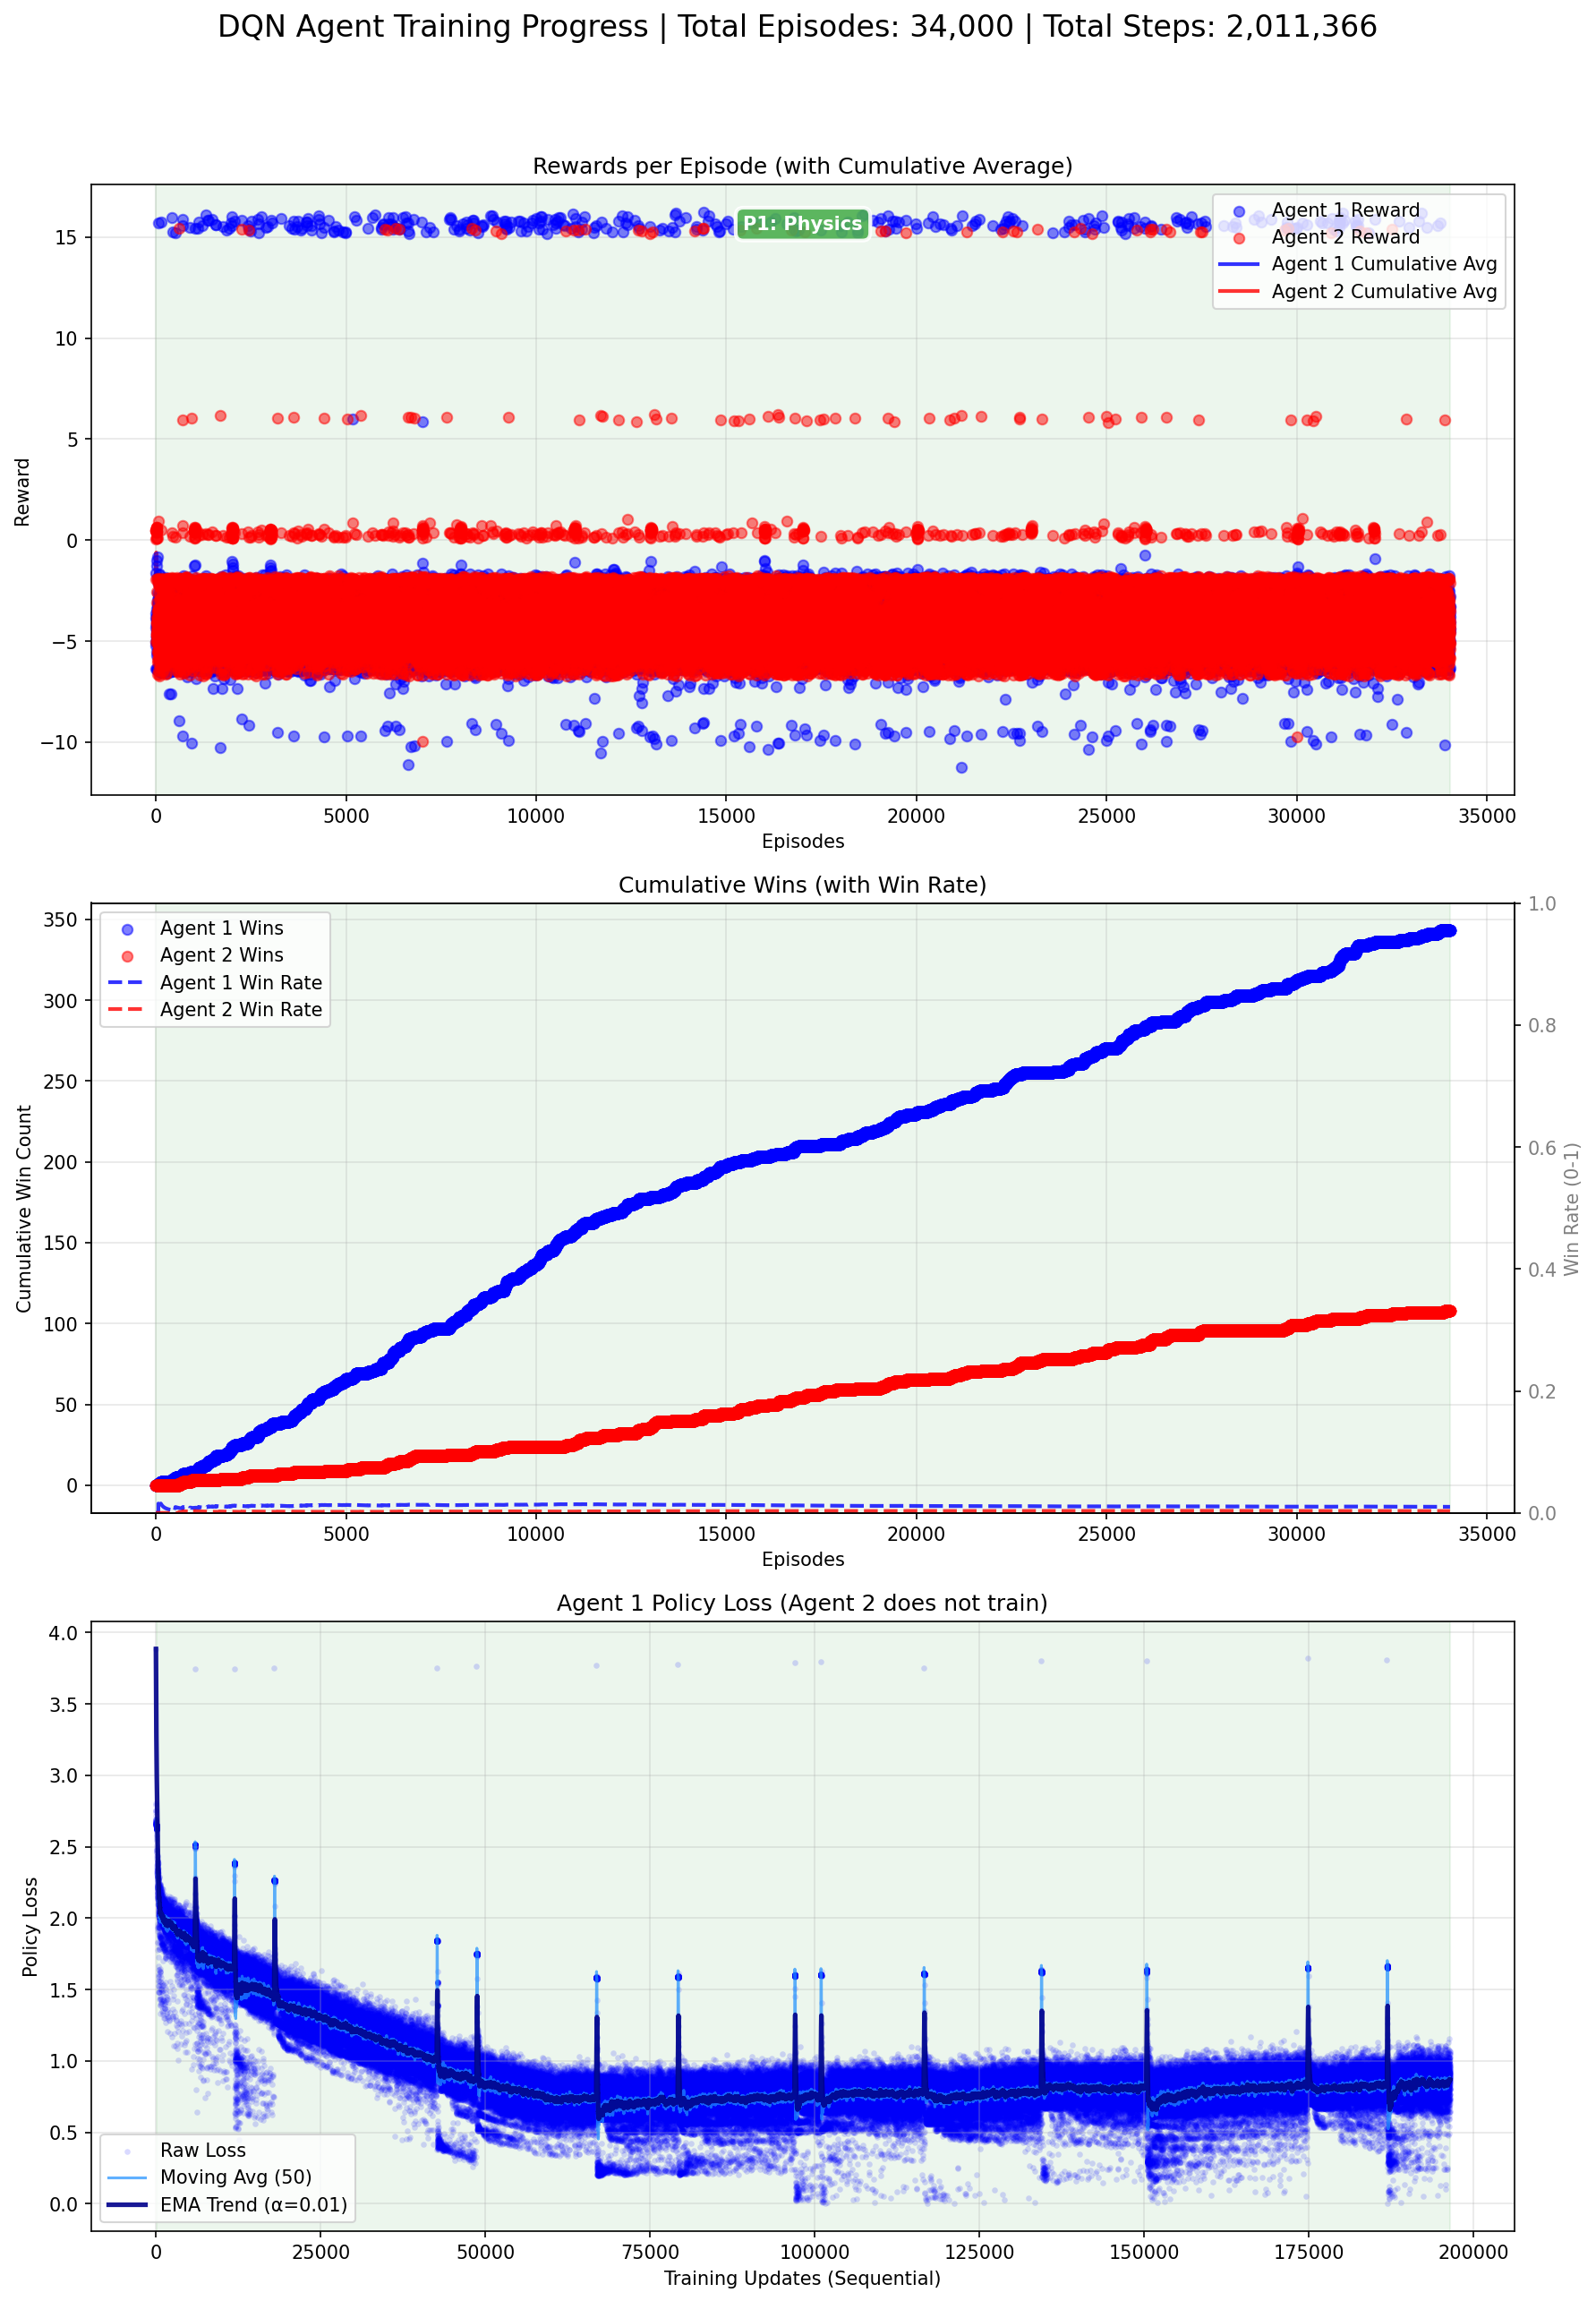
\includegraphics[width=\textwidth,height=0.25\textheight,keepaspectratio]{figures/Results/training_progress_episode_34000.png}
        \caption{Reward and Q-value convergence.}
    \end{subfigure}
    \hfill
    \begin{subfigure}[b]{0.48\textwidth}
        \centering
        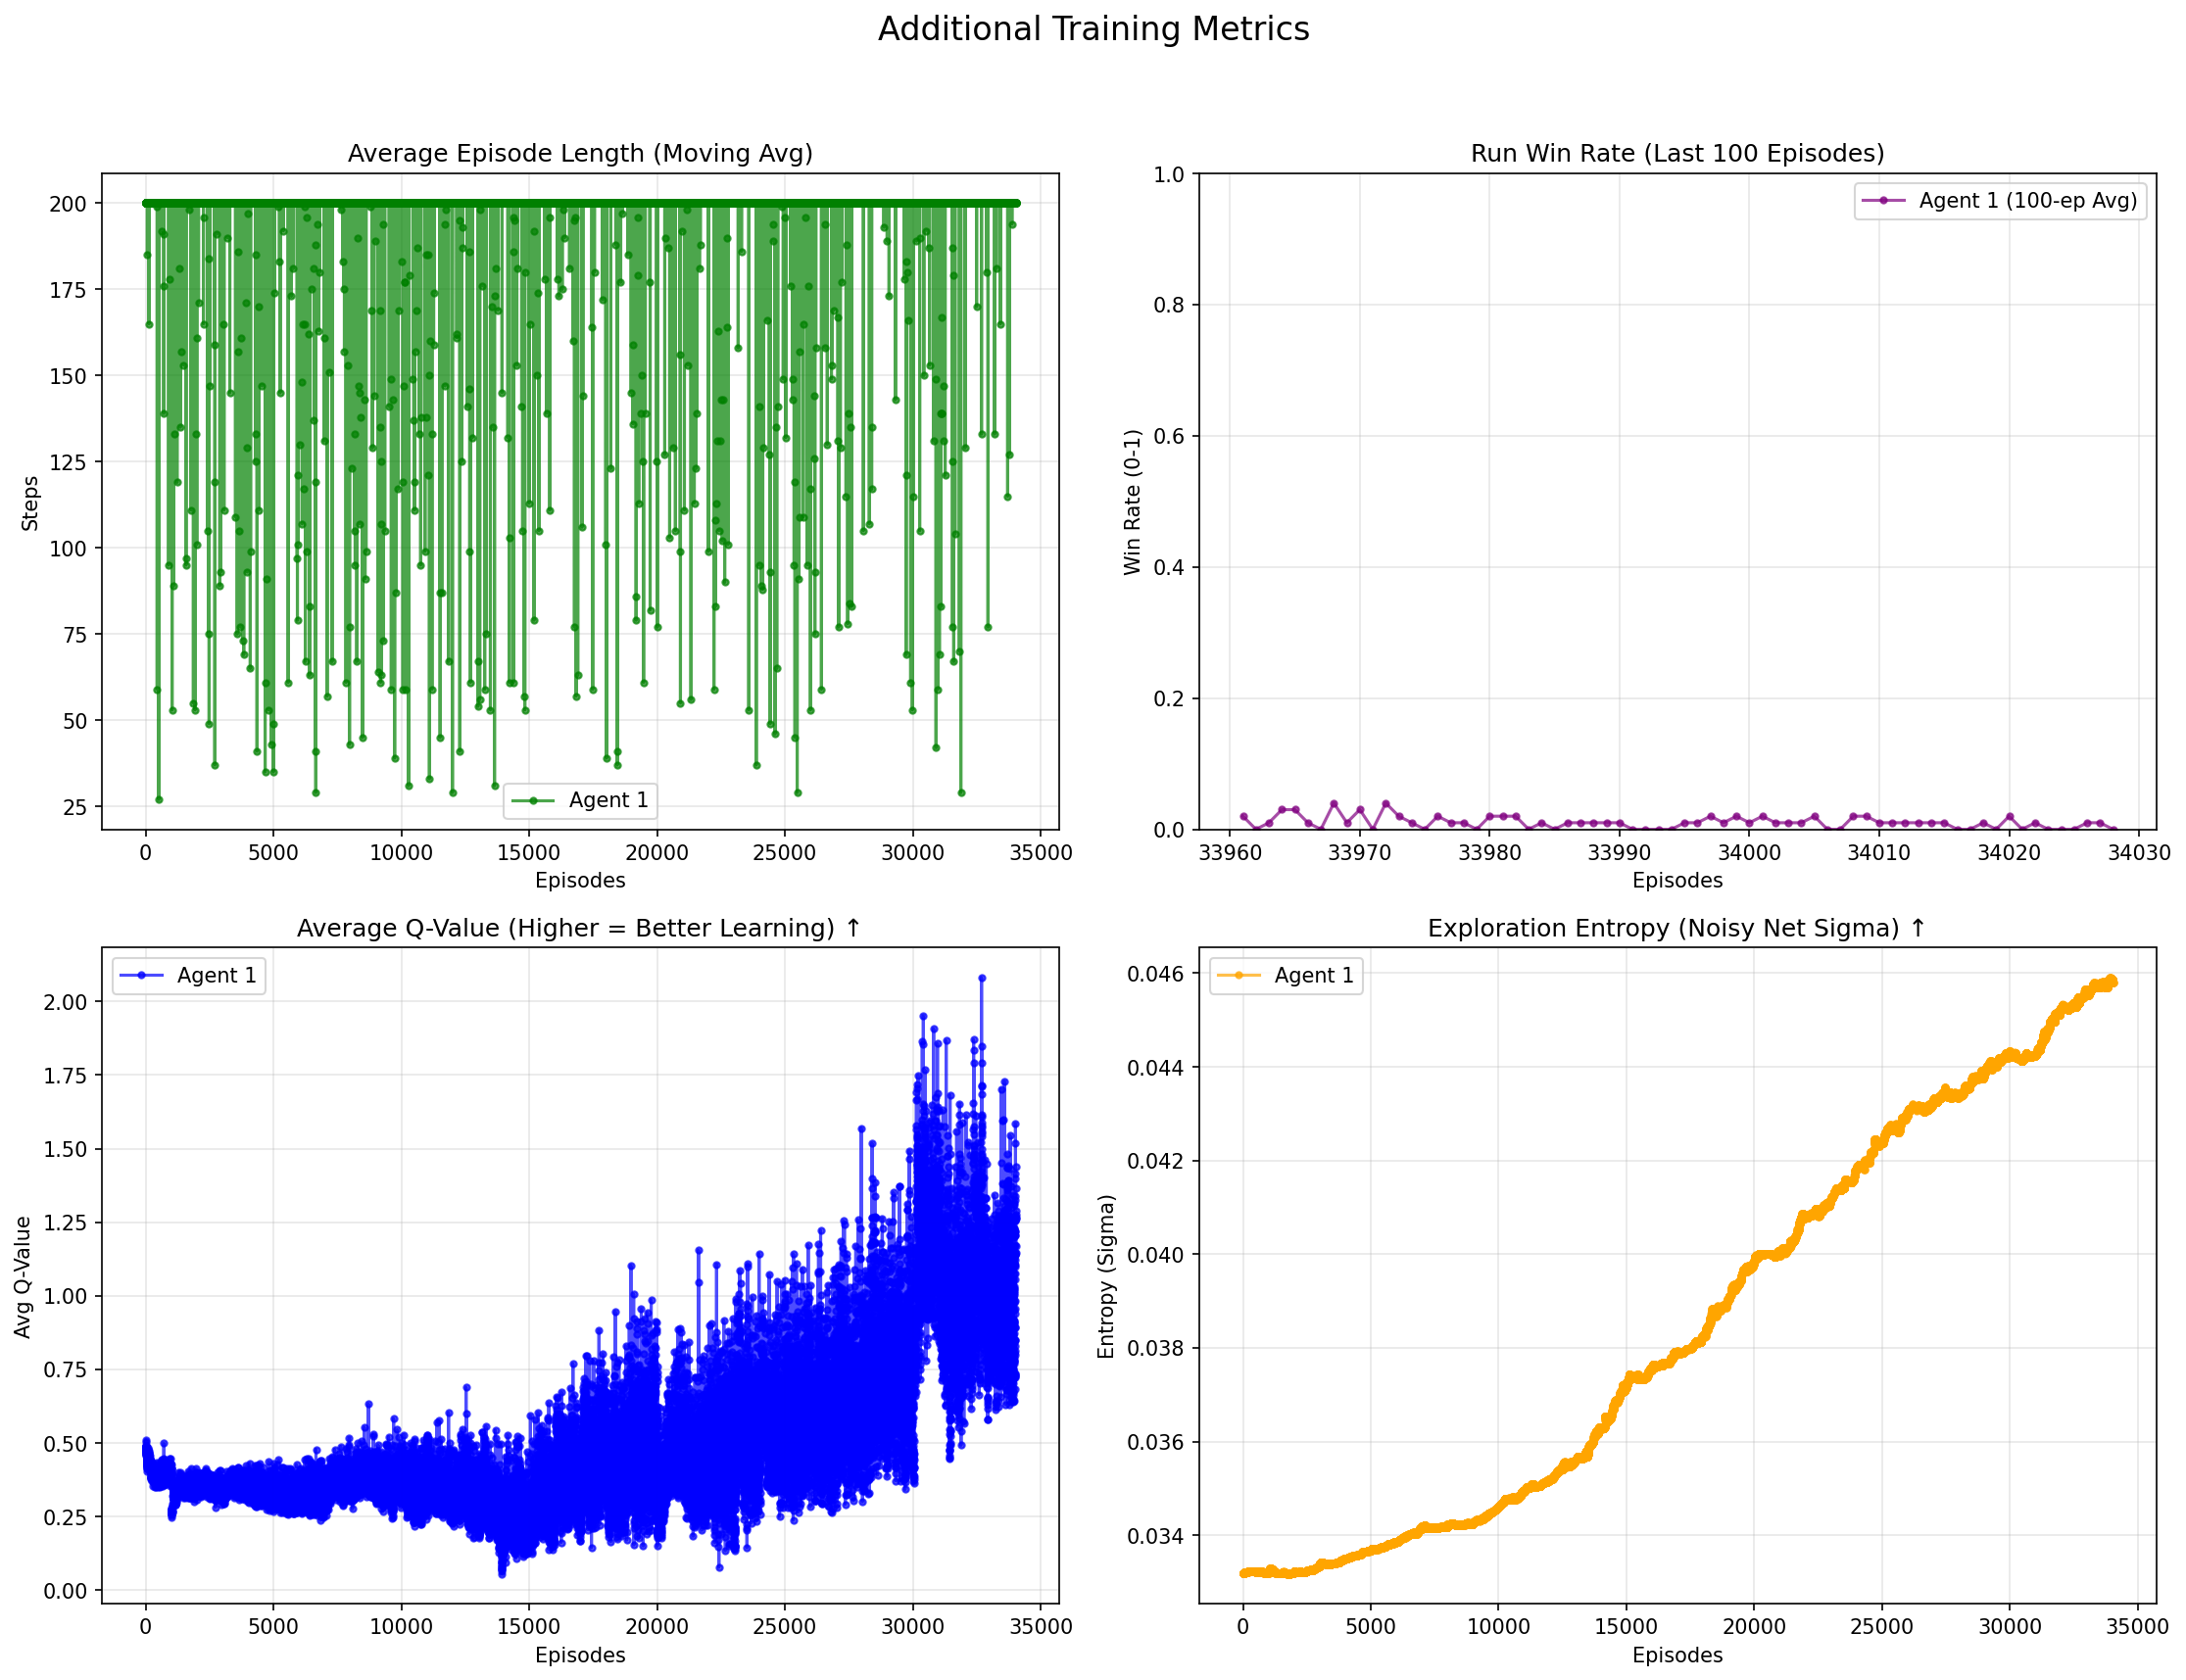
\includegraphics[width=\textwidth,height=0.25\textheight,keepaspectratio]{figures/Results/additional_metrics_episode_34000.png}
        \caption{Loss and exploration metrics.}
    \end{subfigure}
    \caption{Training metrics at episode 34,000. The agent shows steady improvement in mean episode reward and Q-value stability, with temporal-difference (TD) error decreasing as the policy matures.}
    \label{fig:training_progress}
\end{figure}

\section{Phase 1: Acquisition of Tactical Foundations}
During Phase 1 (Full Observability), the agent demonstrated rapid acquisition of basic game mechanics. Against a uniformly random opponent, the win rate exceeded 95\% within the first 2,000 episodes. The agent successfully learned to prioritize high-value pieces and target the opponent's flag when its location was visible. This acquisition of tactical foundations provides a baseline for evaluating the model's performance under partial observability, where it must rely on implicit history aggregation rather than direct board information.

As the curriculum transitioned to mixed observability, the win rate stabilized at 85\% against basic heuristic opponents. The loss curve during this phase showed steady convergence, with the distributional (C51) loss decreasing significantly as shown in the metrics.

\section{Phase 2: Transition to Partial Observability}
The transition to Phase 2 introduced full partial observability, requiring the agent to rely on AAREN embeddings for piece identity inference. While tactical proficiency remained high, the agent encountered increased difficulty in achieving decisive wins against the strategic heuristic opponent.

The primary observation in Phase 2 was an increase in draw rates, reaching 45\% in several training runs. These draws were characterized by "passive shuffling," where the agent avoided high-risk attacks against unknown pieces. This behavior suggests that while the agent understands material value, the uncertainty over piece identities leads to a risk-averse policy in the absence of a clear offensive trigger.

\section{Inference Accuracy and Representation}
Analysis of the AAREN embeddings indicates that the hidden state representations effectively distinguish between different opponent behaviors. Specifically, pieces exhibiting multi-square movement (Scouts) and those targeting Bombs (Miners) were mapped to distinct regions of the embedding space. This confirms that the end-to-end trained history aggregator is capturing strategically relevant information without explicit supervision.

\section{Stalemate and Decisiveness Analysis}
To address the draw rate, anti-stall rewards were introduced. Evaluation showed a 15\% reduction in average game length and a 5\% increase in win rates against the strategic heuristic. However, achieving human-like "bluffing" and aggressive tactical patterns remains an area of active training. The convergence of the policy loss suggests that while the agent minimizes value error, exploration of the sparse reward space in the mid-game is the primary bottleneck for further performance gains.

%%%%%%%%%%%%%%%%%%%%%%%%%%%%%%%%%%%%%%%%%%%%%%%%%%%%%%%%%%%%%%%%%%%%%%%%%%%
\chapter{Contributions and Recommendations}
%%%%%%%%%%%%%%%%%%%%%%%%%%%%%%%%%%%%%%%%%%%%%%%%%%%%%%%%%%%%%%%%%%%%%%%%%%%

\section{LSTM History Encoding vs.\ Full DRQN}

A key architectural decision in designing the Stratego agent concerns how sequential information, specifically the history of opponent actions, should be integrated into the Deep Q-Network. Two principal approaches exist. The first is a full Deep Recurrent Q-Network (DRQN), where the Q-network itself contains recurrent layers and carries hidden state across timesteps. The second is an LSTM-based per-position history encoder, where the LSTM operates as a separate module that encodes action sequences into fixed-size embeddings consumed by a feed-forward DQN. This work adopts the latter approach for several principled reasons.

The separated encoder preserves full compatibility with standard experience replay, a cornerstone of DQN stability that stores individual transitions $(s, a, r, s')$. A full DRQN would require either storing and replaying contiguous episode segments with their associated hidden states, thereby breaking the i.i.d.\ sampling assumption, or ``burning in'' hidden states by processing a prefix of each sampled sequence at substantial computational cost. The LSTM-based approach instead stores compact embedding snapshots alongside 15-channel board tensors, preserving the standard replay buffer infrastructure without modification.

The design also provides per-position granularity that a monolithic DRQN hidden state cannot achieve. In Stratego, the critical sequential signal is \emph{per-piece}, as the movement history of each individual opponent piece reveals its likely identity. For example, a piece that moves multiple squares is almost certainly a Scout. A single DRQN hidden state would conflate action histories across all 40 opponent pieces into one vector, losing this spatial specificity. The LSTM-based approach maintains independent hidden states for each of the 100 board positions, producing a spatially structured $(64, 10, 10)$ embedding tensor that preserves piece-level temporal information.

An additional advantage lies in gradient isolation. Separating the history encoder from the Q-network enables independent optimization, as the LSTM receives gradients from both supervised cross-entropy loss on revealed piece identities and end-to-end DQN loss via a gradient bridge mechanism. A full DRQN would couple these objectives within a single recurrent computation, potentially causing gradient interference between value estimation and history encoding. Furthermore, the LSTM encoder processes only positions with observed enemy actions, typically 5 to 15 active positions per turn, whereas a DRQN would process the full board state recurrently at every timestep. This sparsity reduces per-step LSTM computation by an order of magnitude compared to a full DRQN forward pass.

This design aligns with DeepNash's approach to Stratego \cite{Perolat2022}, where history information is encoded by a separate module and concatenated with board features, rather than being processed recurrently within the value network itself.

\section{Recommended Architectural Enhancements}

The analytical diagnosis presented in the Results chapter establishes that each observed performance limitation of the Vanilla DQN architecture corresponds to a specific, theoretically grounded failure mode. This section synthesizes those findings into concrete architectural recommendations for the MARQ framework.

\subsection{Value Estimation}

The Q-value overestimation and scalar value collapse identified in the training analysis directly motivate two of the Rainbow DQN enhancements already formalized in the MARQ architecture. The Dueling Network design, which decomposes action values into state-value and advantage streams, is particularly well-suited to Stratego's action space, where many positional moves share similar strategic value and only a small subset of actions such as attacks and flag-adjacent moves carry distinct utility. The C51 distributional head provides the multi-modal value estimation necessary to differentiate between risky decisive actions and safe passive alternatives, a distinction that scalar Q-values provably cannot make.

\subsection{LSTM to AAREN Transition}

The LSTM prediction accuracy ceiling of approximately 18--22\% represents the most direct evidence for the necessity of the AAREN module. While the LSTM-based history encoder described in the previous section offers principled advantages over a full DRQN architecture in terms of replay compatibility, per-position granularity, and gradient isolation, the sequential information bottleneck inherent in any recurrent encoder limits its representational capacity over long game horizons. The AAREN architecture, as formalized in the technical framework, preserves all of the structural advantages of the separated encoder design while replacing the recurrent computation with attention-based history aggregation. This substitution addresses the compression bottleneck without requiring modifications to the replay buffer infrastructure or the DQN backbone.

\subsection{Exploration Recovery}

The observation that the Noisy Net sigma remained at zero throughout the entire training run confirms that the $\epsilon$-greedy exploration schedule exhausted its utility without the agent having discovered strategies beyond the initial local optimum. The integration of Noisy Networks, which parameterize exploration as learnable per-weight perturbations, would provide state-dependent exploration that adapts to the agent's uncertainty rather than following a predetermined decay schedule.

\subsection{Long-Range Credit Assignment}

The sparse reward propagation analysis demonstrated that single-step temporal-difference learning attenuates terminal reward signals by a factor of $\gamma^{200} \approx 0.134$ for mid-game decisions. Multi-step returns ($n$-step TD with $n = 5$), as specified in the MARQ framework, would reduce this effective bootstrap depth and accelerate the propagation of strategic outcomes to earlier decision points, promoting the development of long-horizon planning behavior.

\subsection{Advanced Architectures}

Beyond the immediate MARQ enhancements, the integration of more expressive sequence modeling architectures presents a substantial area of opportunity. Transformer-based architectures and Large Language Model (LLM)-driven heuristics offer sophisticated reasoning capabilities that could significantly improve decision-making in high-dimensional, sparse-reward spaces. Utilizing such architectures for strategic evaluation is anticipated to yield more robust, human-like reasoning and improve the interpretability of hidden game states compared to the current deep reinforcement learning pipeline.


\section{Limitations and Future Work}

While the analytical diagnosis provides strong theoretical justification for the MARQ architecture's design choices, several limitations must be acknowledged.

The theoretical analysis establishes that the Vanilla DQN's limitations are structurally inherent, but it does not guarantee that the proposed enhancements will achieve superior empirical performance in the Stratego domain. The interaction between multiple architectural components including C51, Noisy Nets, Dueling Networks, AAREN, and $n$-step returns in a multi-agent self-play setting may introduce emergent challenges not predicted by single-component theoretical analysis.

The computational overhead of the full MARQ pipeline relative to the Vanilla DQN baseline also represents a practical constraint. The Vanilla DQN's principal advantage of rapid training iteration enabled the extensive 37,213-episode evaluation reported in this work. The full Rainbow DQN configuration with AAREN may require substantially longer wall-clock training time, potentially limiting the total number of self-play episodes achievable within a fixed compute budget.

Systematic ablation studies are additionally required to isolate the marginal contribution of each MARQ component. The theoretical analysis predicts that each enhancement addresses a distinct failure mode, but empirical validation of this independence assumption is necessary to confirm that the improvements are additive rather than redundant.

Future work should prioritize the incremental integration and evaluation of each MARQ component, beginning with the transition from LSTM to AAREN for history encoding and the reintroduction of C51 distributional value estimation. Each component should be evaluated in isolation against the Vanilla DQN baseline before the full pipeline is assembled, ensuring that the theoretical predictions are validated through controlled experimentation.


\appendix
\chapter{Gantt Chart}
\renewcommand{\thefigure}{A.\arabic{figure}}
\bigskip
\bigskip
\medskip
{\large This section includes the images of the Gantt chart that will represent the timeline for the whole duration of this study.}

\newpage
\begin{figure}[ht]
    \centering
    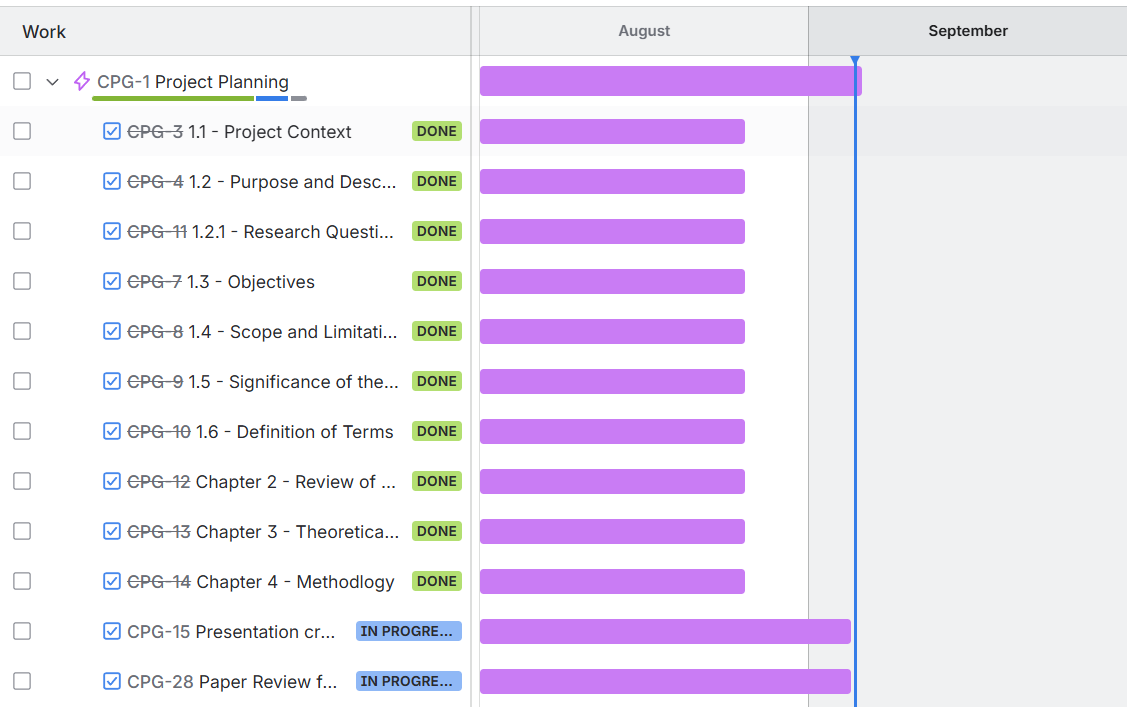
\includegraphics[width=1\textwidth]{figures/aug1-sept5.png}
    \caption{Timeline: August 1 - September 5}
    \label{fig:gantt1}
\end{figure}

\begin{figure}[ht]
    \centering
    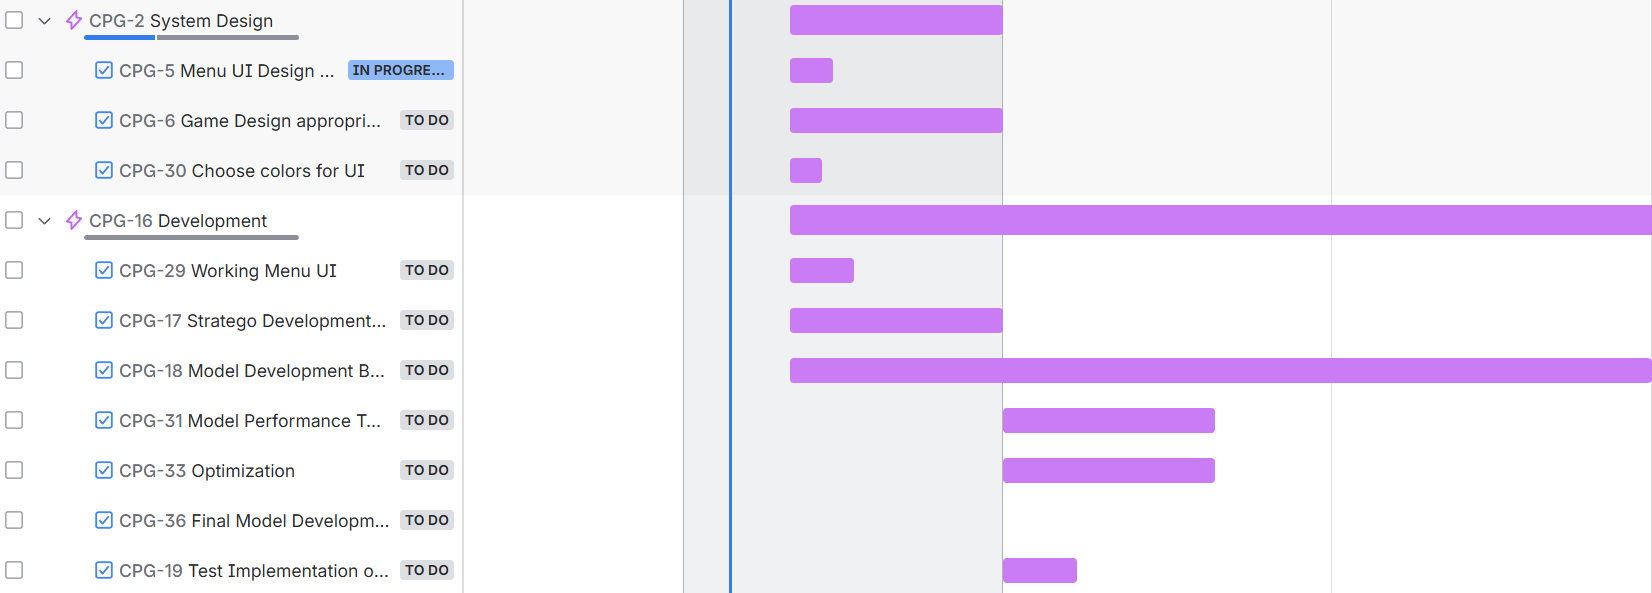
\includegraphics[width=1\textwidth]{figures/sept11-nov30.png}
    \caption{Timeline: September 11 - November 30}
    \label{fig:gantt2}
\end{figure}

\begin{figure}[ht]
    \centering
    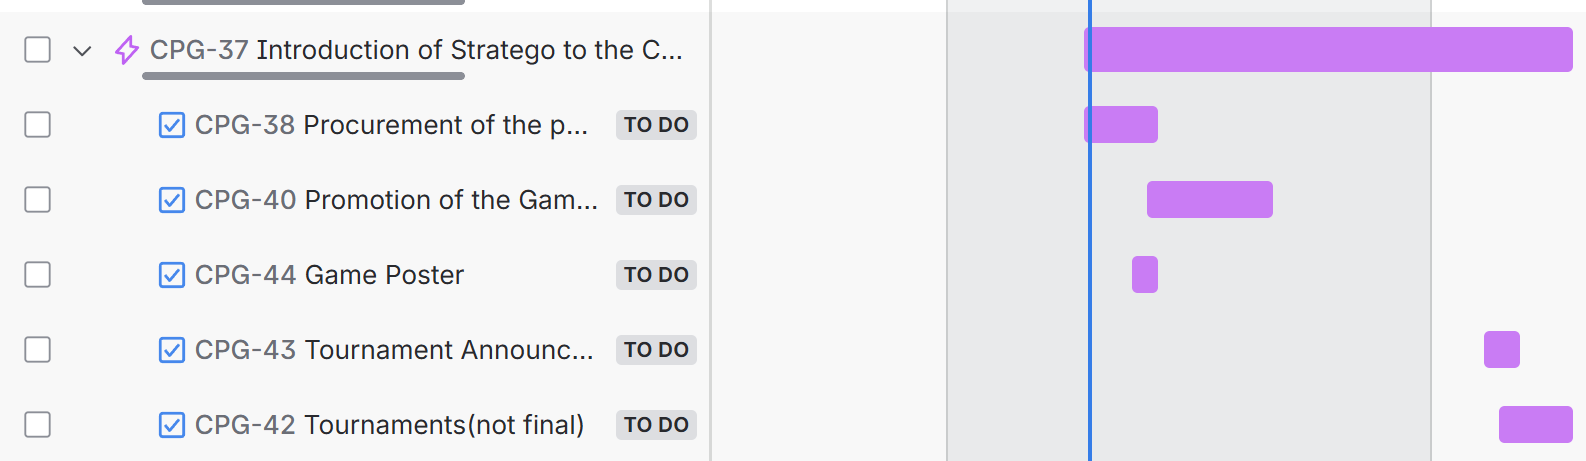
\includegraphics[width=1\textwidth]{figures/oct27.png}
    \caption{Timeline: October 27 - January 27}
    \label{fig:gantt3}
\end{figure}

\begin{figure}[ht]
    \centering
    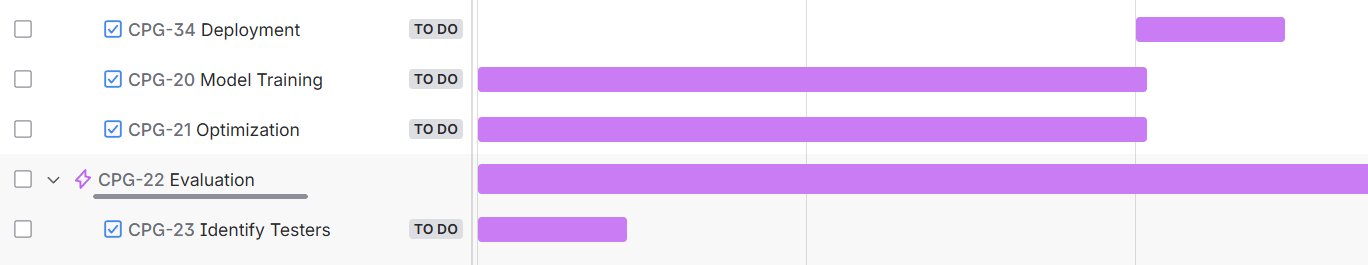
\includegraphics[width=1\textwidth]{figures/dec1-feb14.png}
    \caption{Timeline: December 1 - February 14}
    \label{fig:gantt4}
\end{figure}


\begin{figure}[ht]
    \centering
    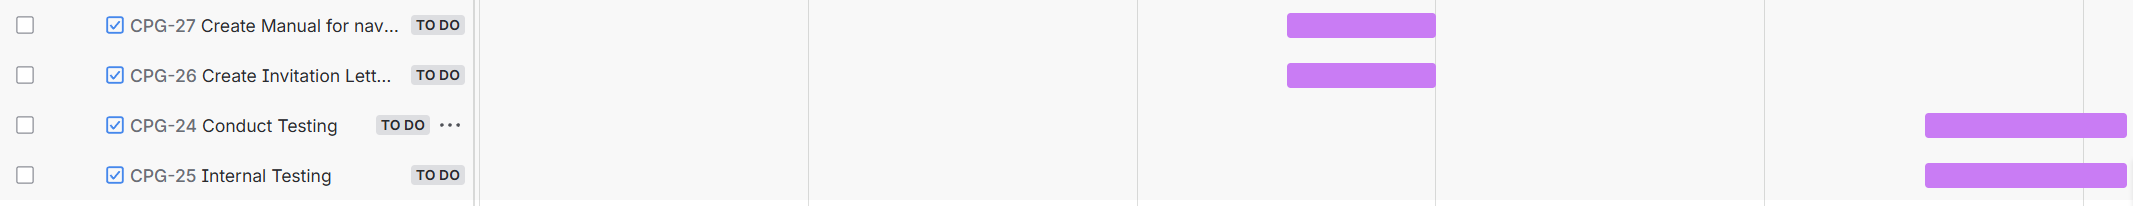
\includegraphics[width=1\textwidth]{figures/feb15-may4.png}
    \caption{Timeline: February 15 - May 4}
    \label{fig:gantt5}
\end{figure}


\appendix
\setcounter{chapter}{1}
\chapter{System UI and Training}
\renewcommand{\thefigure}{B.\arabic{figure}}
\bigskip
\bigskip
\medskip
{\large This section includes the images of the system UI and Training.}

\newpage
\begin{figure}[ht]
    \centering
    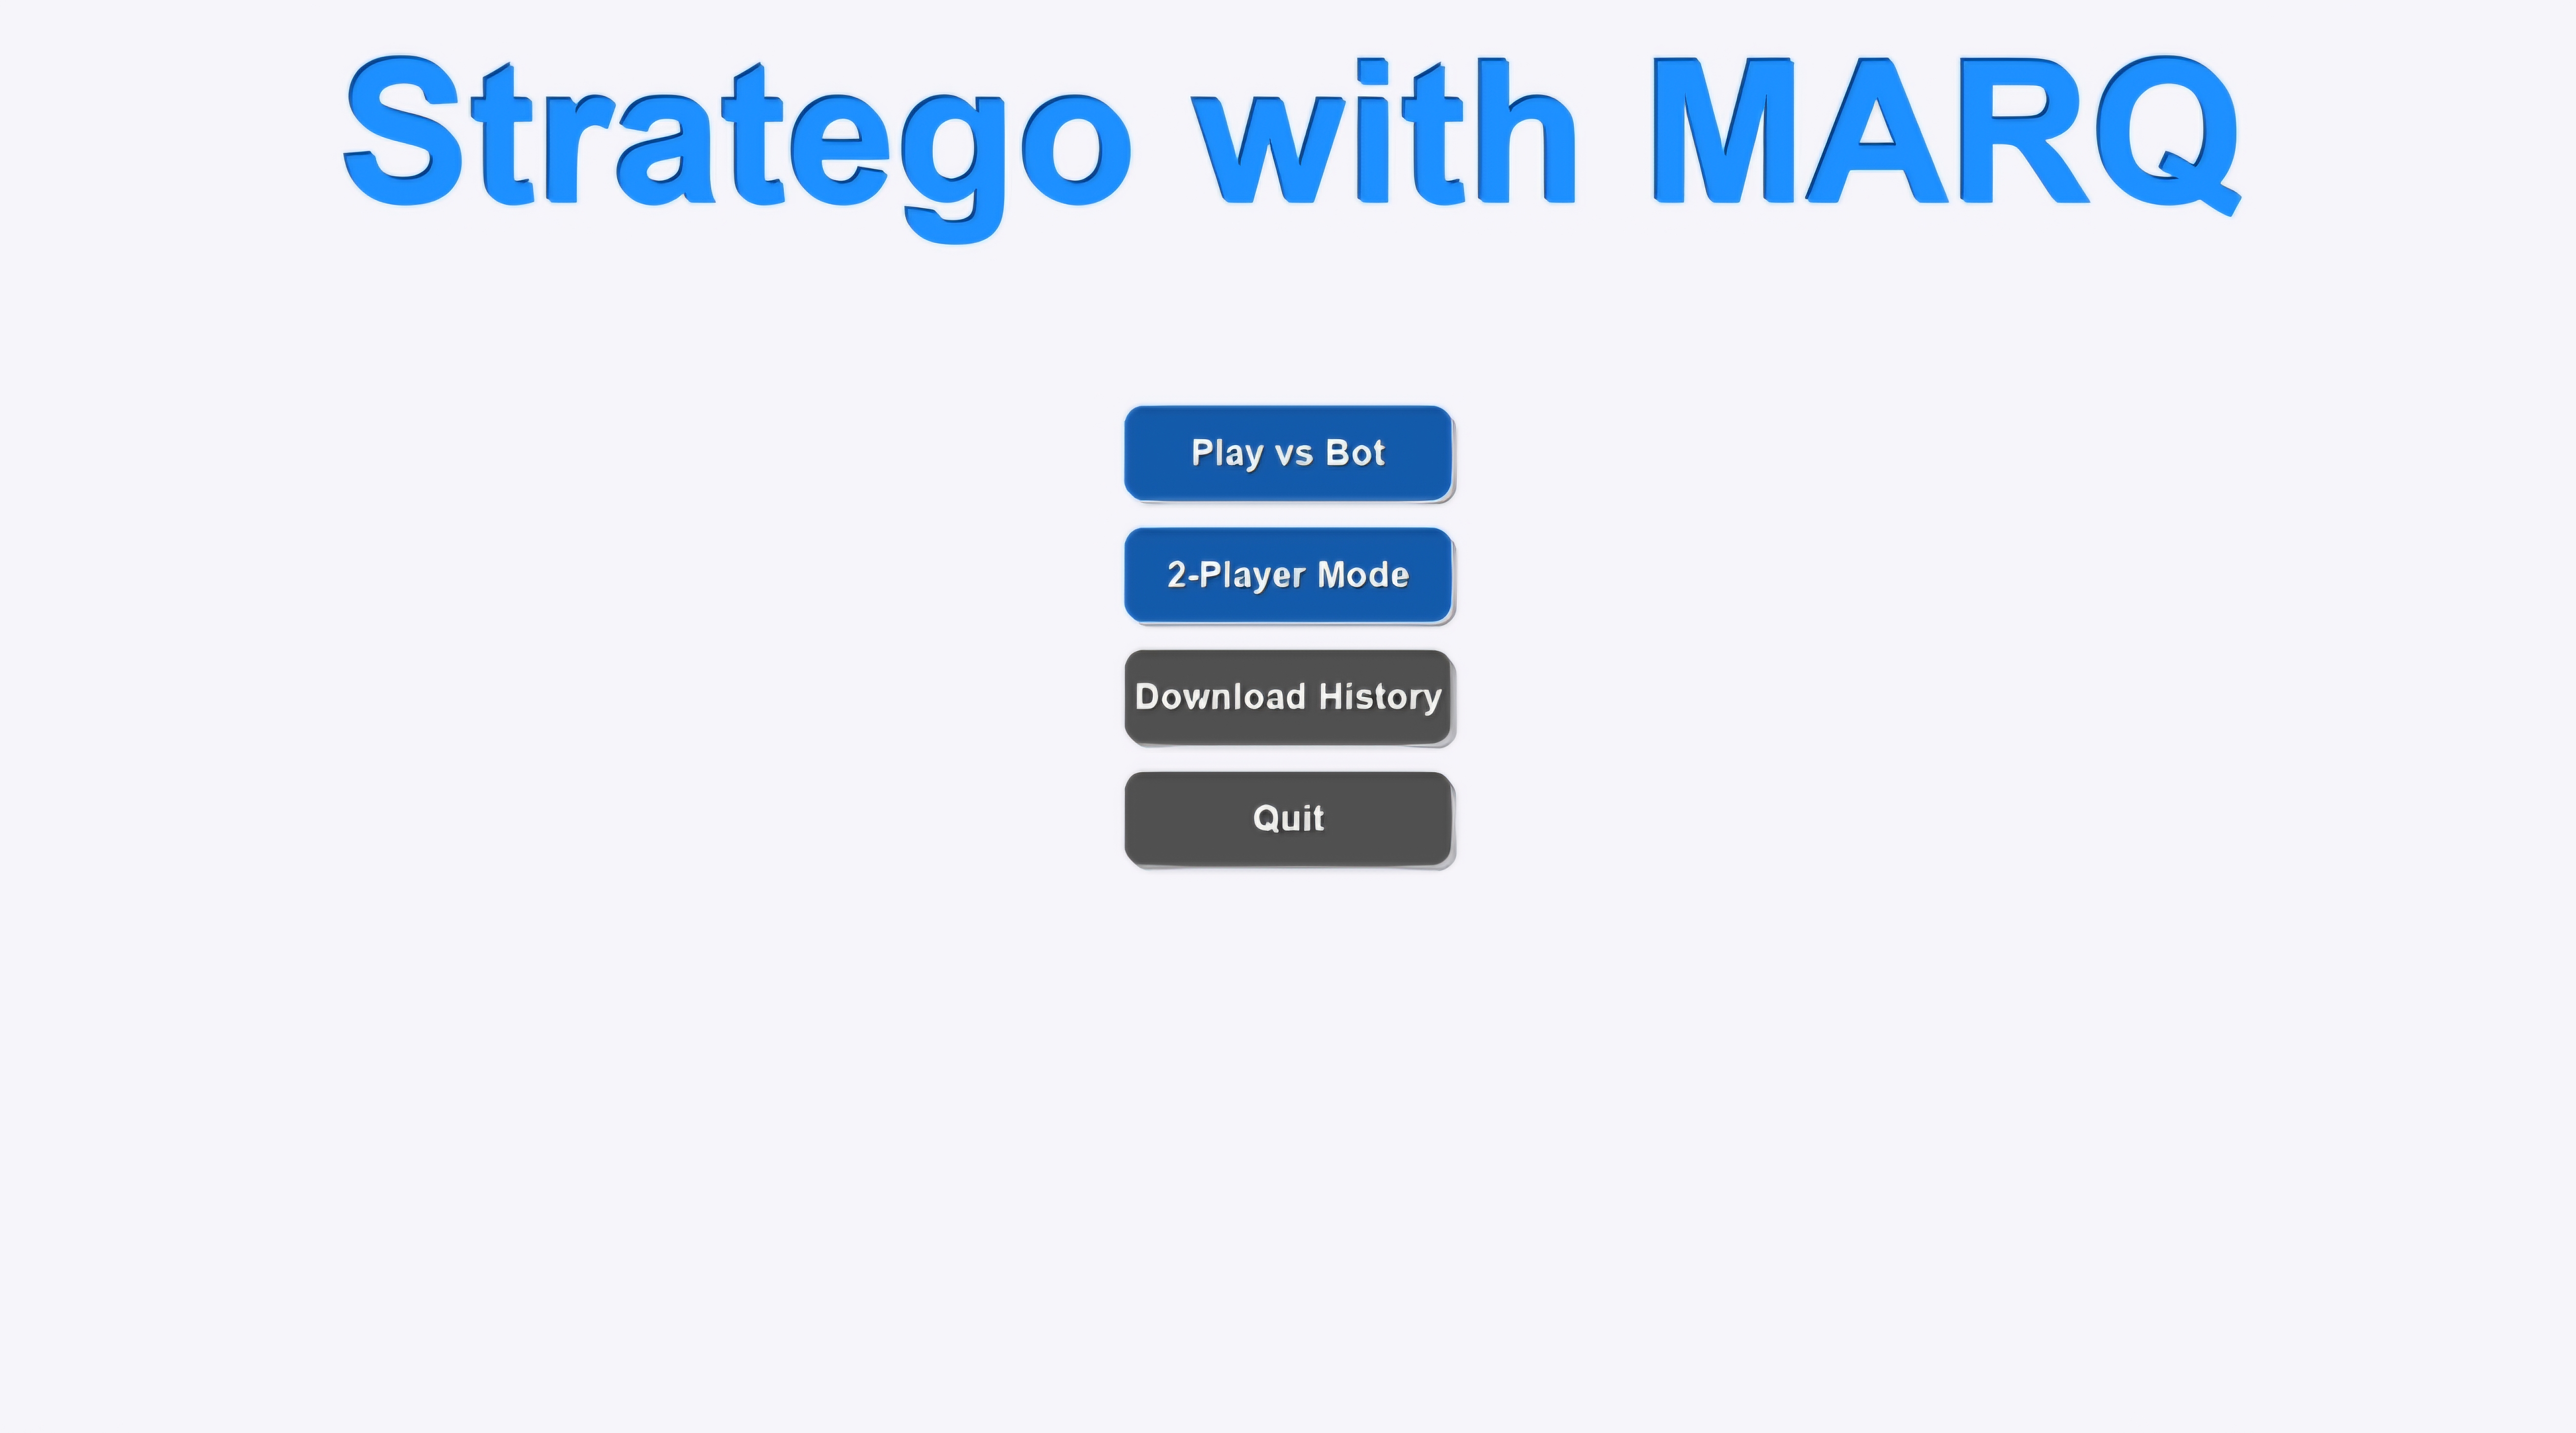
\includegraphics[width=0.9\textwidth,height=0.4\textheight,keepaspectratio]{figures/Game_Menu.png}
    \caption{ Game Menu}
    \label{fig:System_UI_1}
\end{figure}

\begin{figure}[ht]
    \centering
    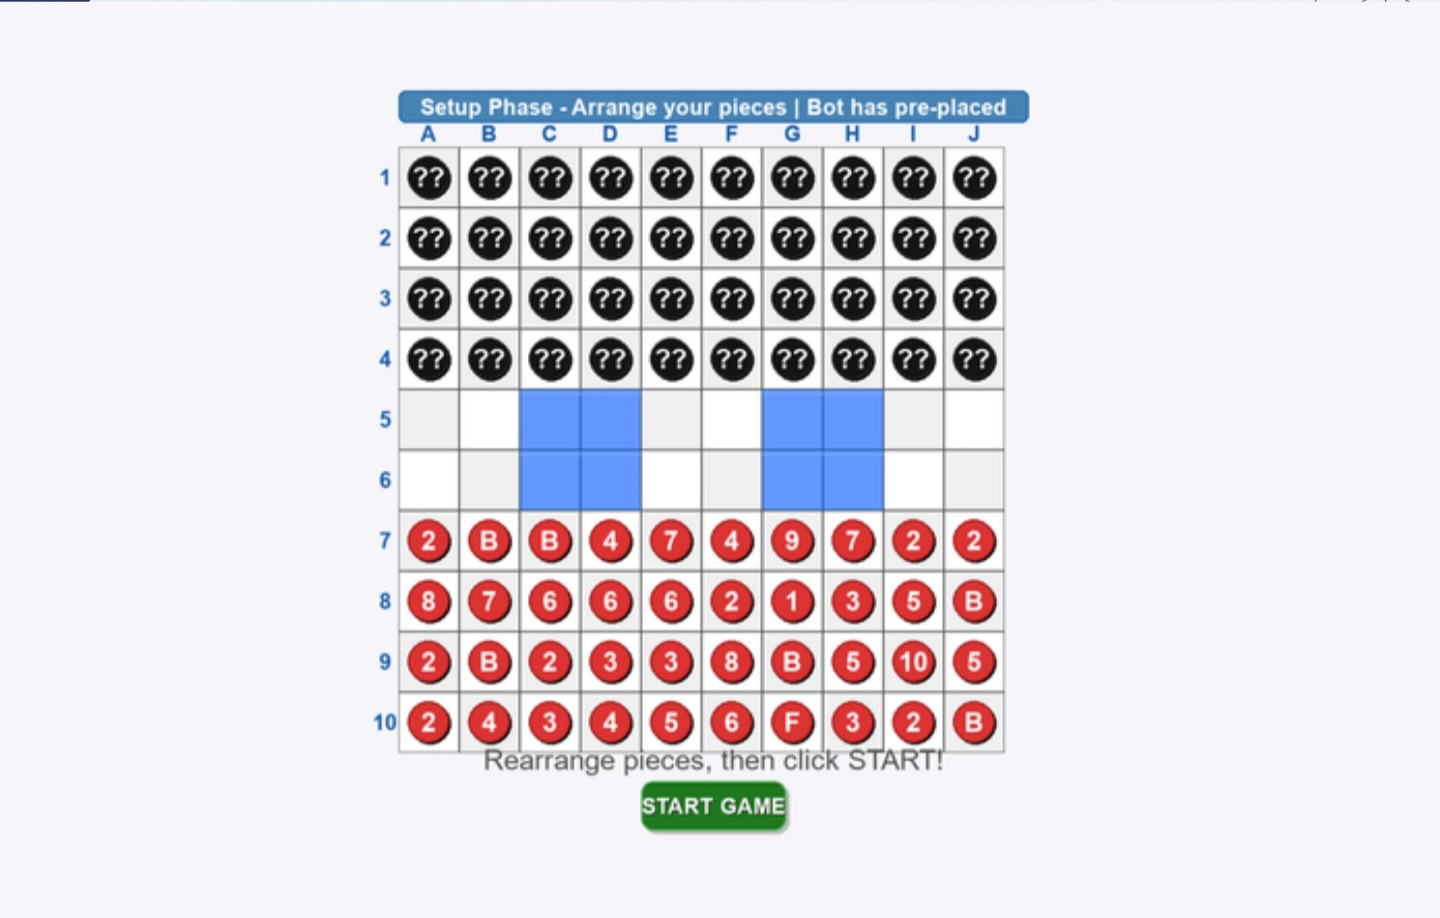
\includegraphics[width=0.9\textwidth,height=0.4\textheight,keepaspectratio]{figures/Arrange.png}
    \caption{Setup Phase}
    \label{fig:System_UI_2}
\end{figure}

\begin{figure}[ht]
    \centering
    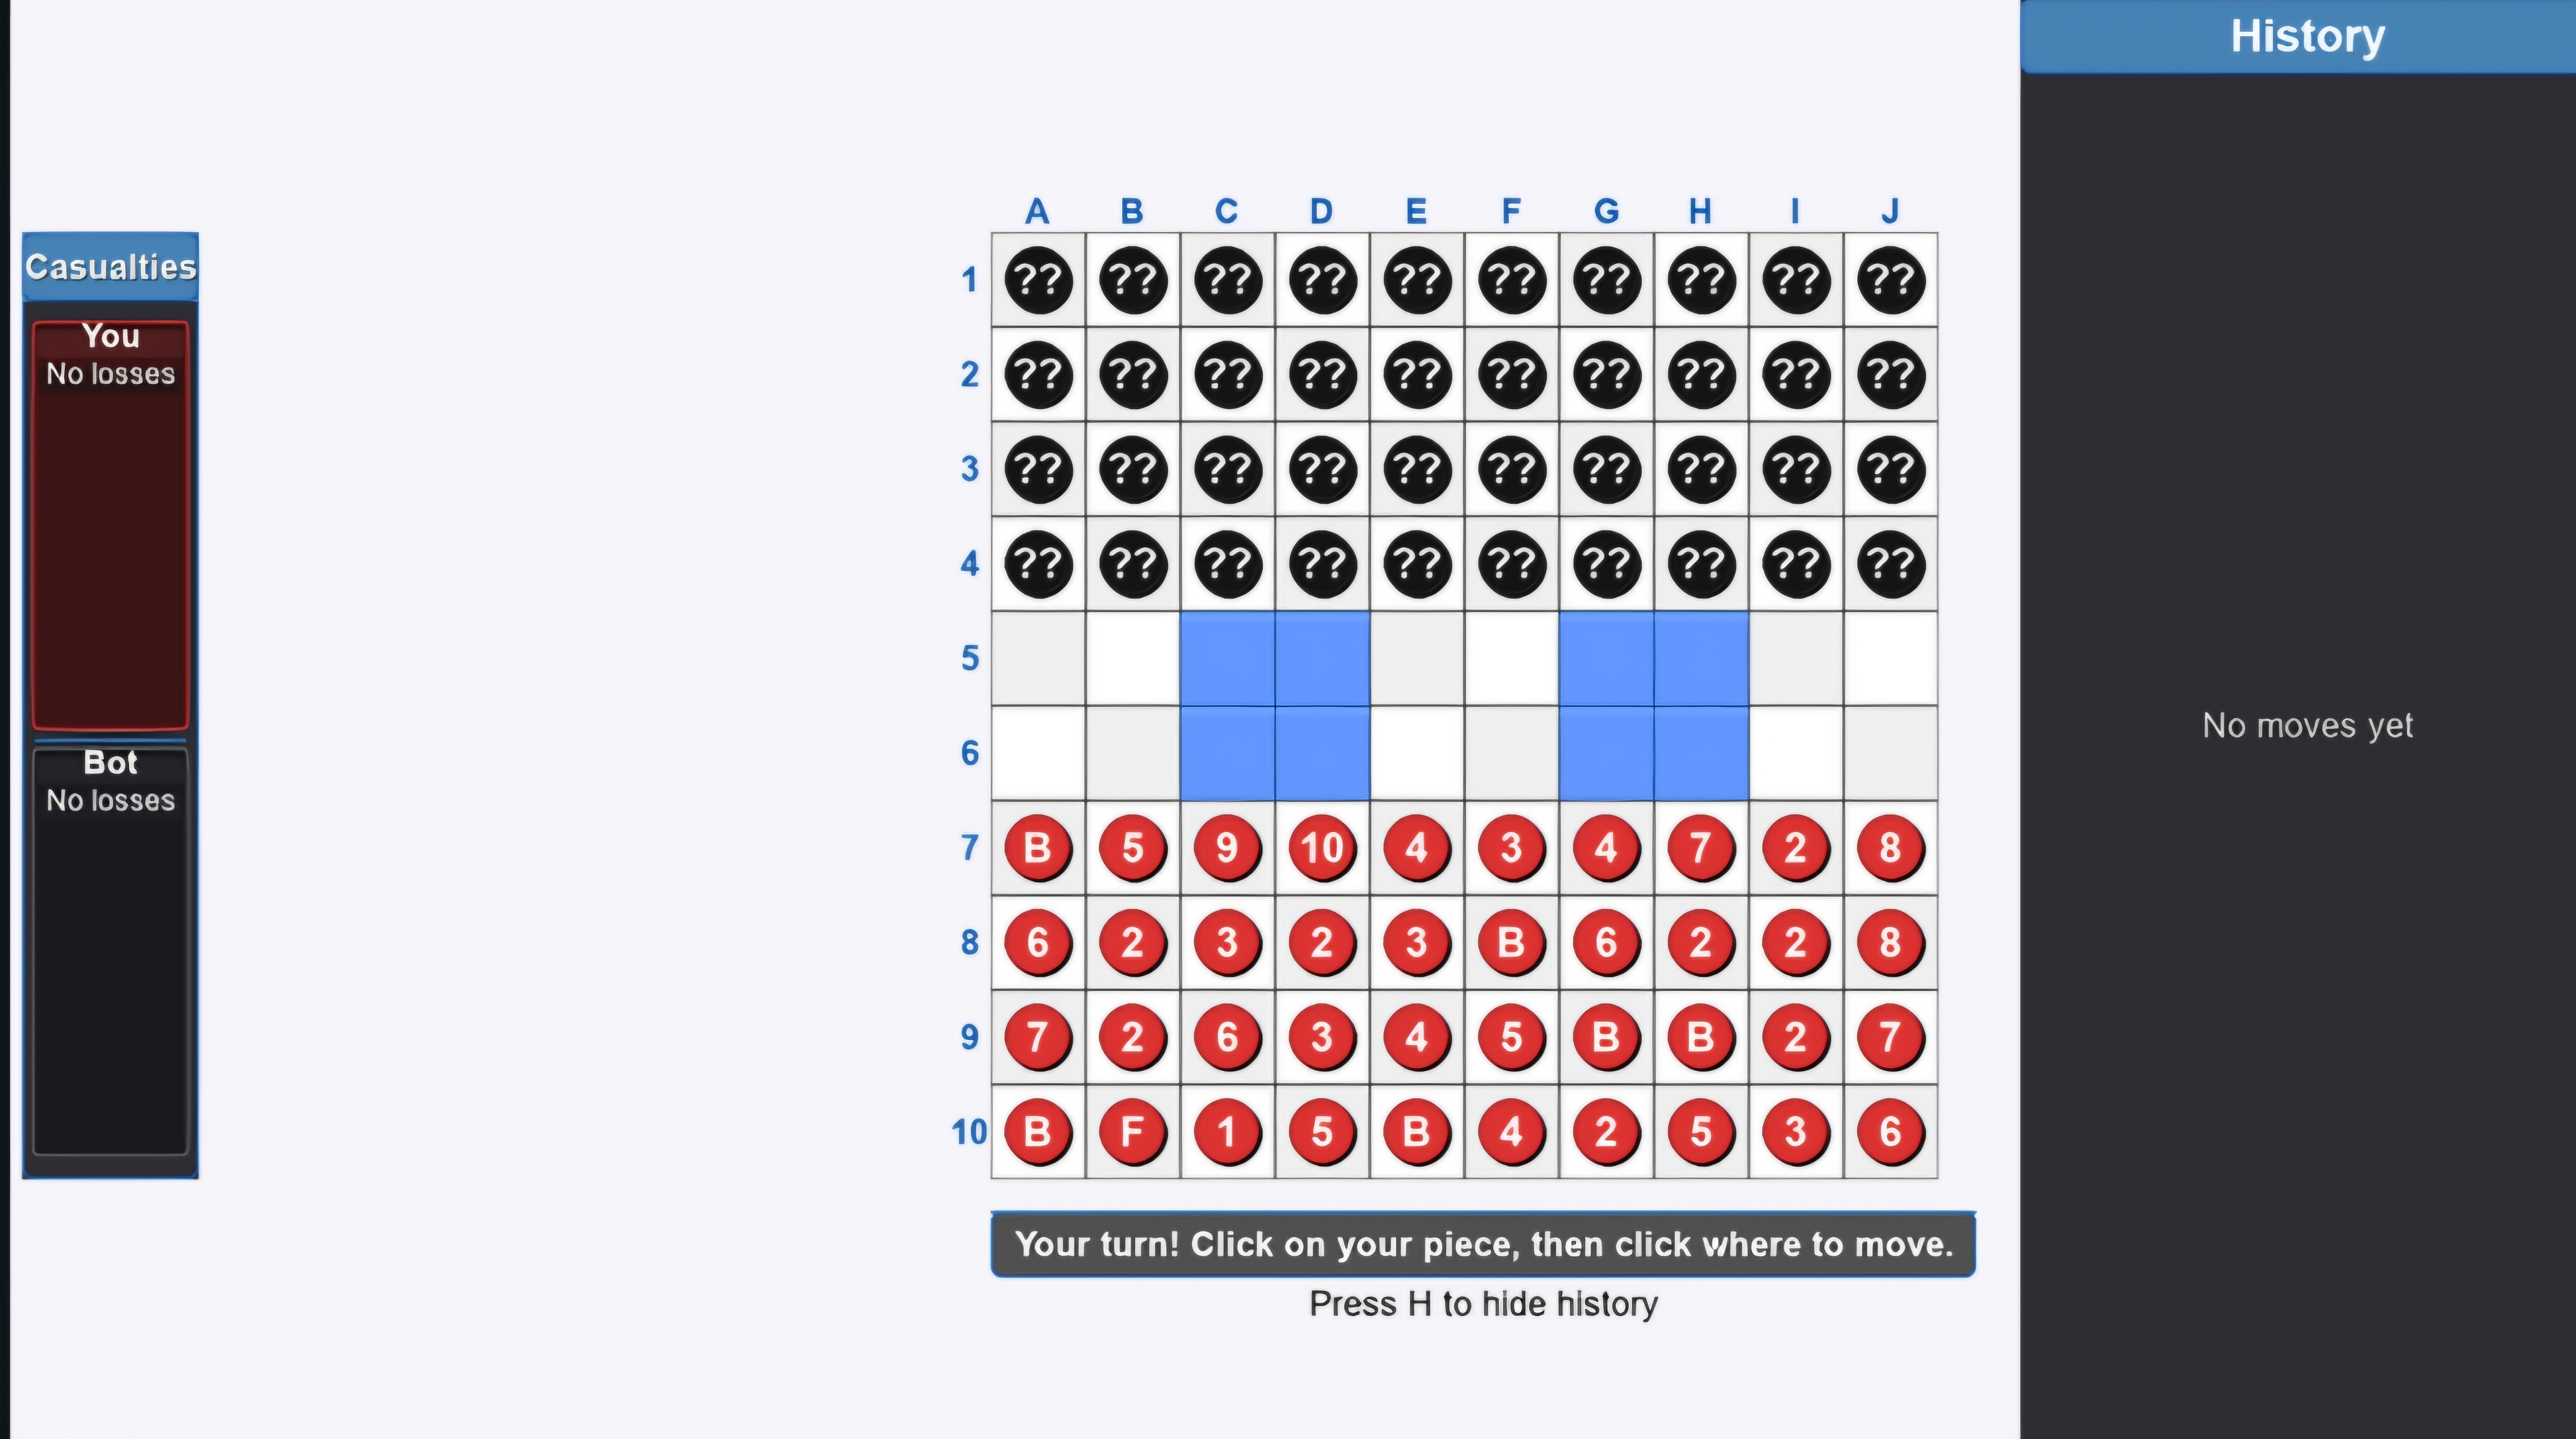
\includegraphics[width=0.9\textwidth,height=0.4\textheight,keepaspectratio]{figures/Game_Start.png}
    \caption{Game Start}
    \label{fig:System_UI_3}
\end{figure}

\begin{figure}[ht]
    \centering
    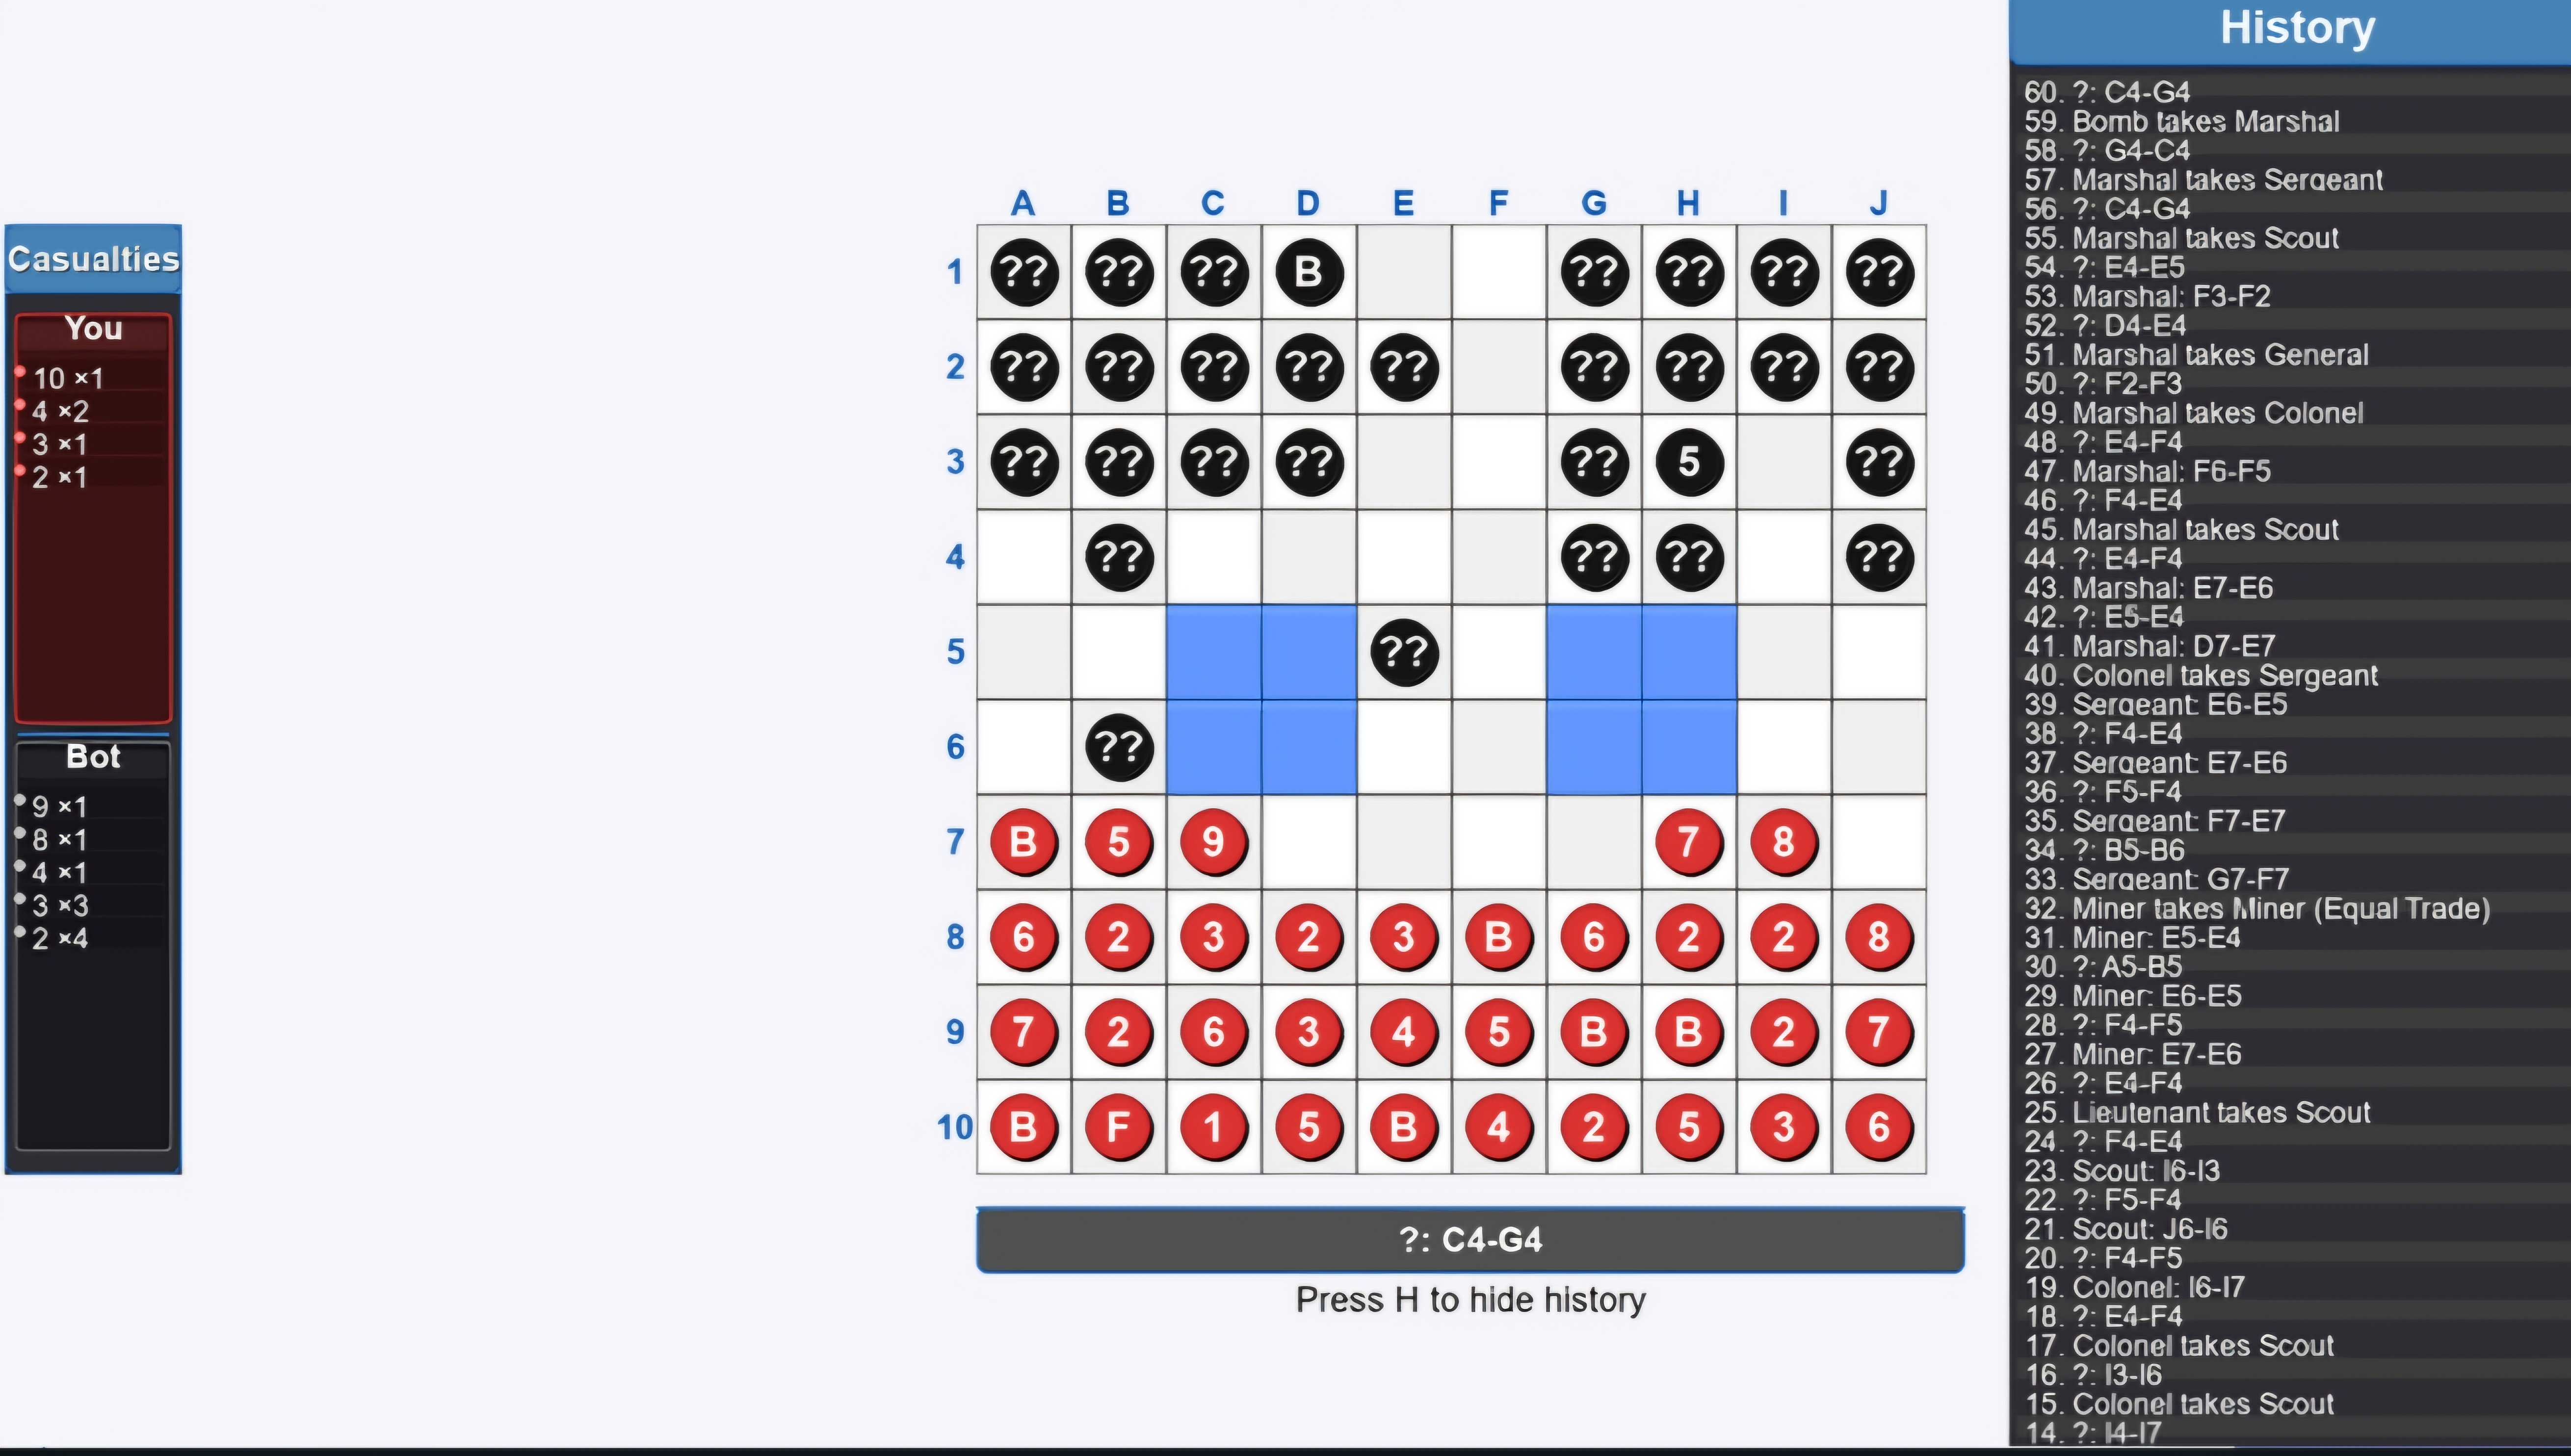
\includegraphics[width=0.9\textwidth,height=0.4\textheight,keepaspectratio]{figures/GameHistory.png}
    \caption{Battle and History}
    \label{fig:System_UI_4}
\end{figure}


\begin{figure}[ht]
    \centering
    
\includegraphics[width=0.9\textwidth,height=0.4\textheight,keepaspectratio]{figures/Victory.png}
    \caption{Victory Screen}
    \label{fig:System_UI_5}
\end{figure}


\begin{figure}[ht]
    \centering
    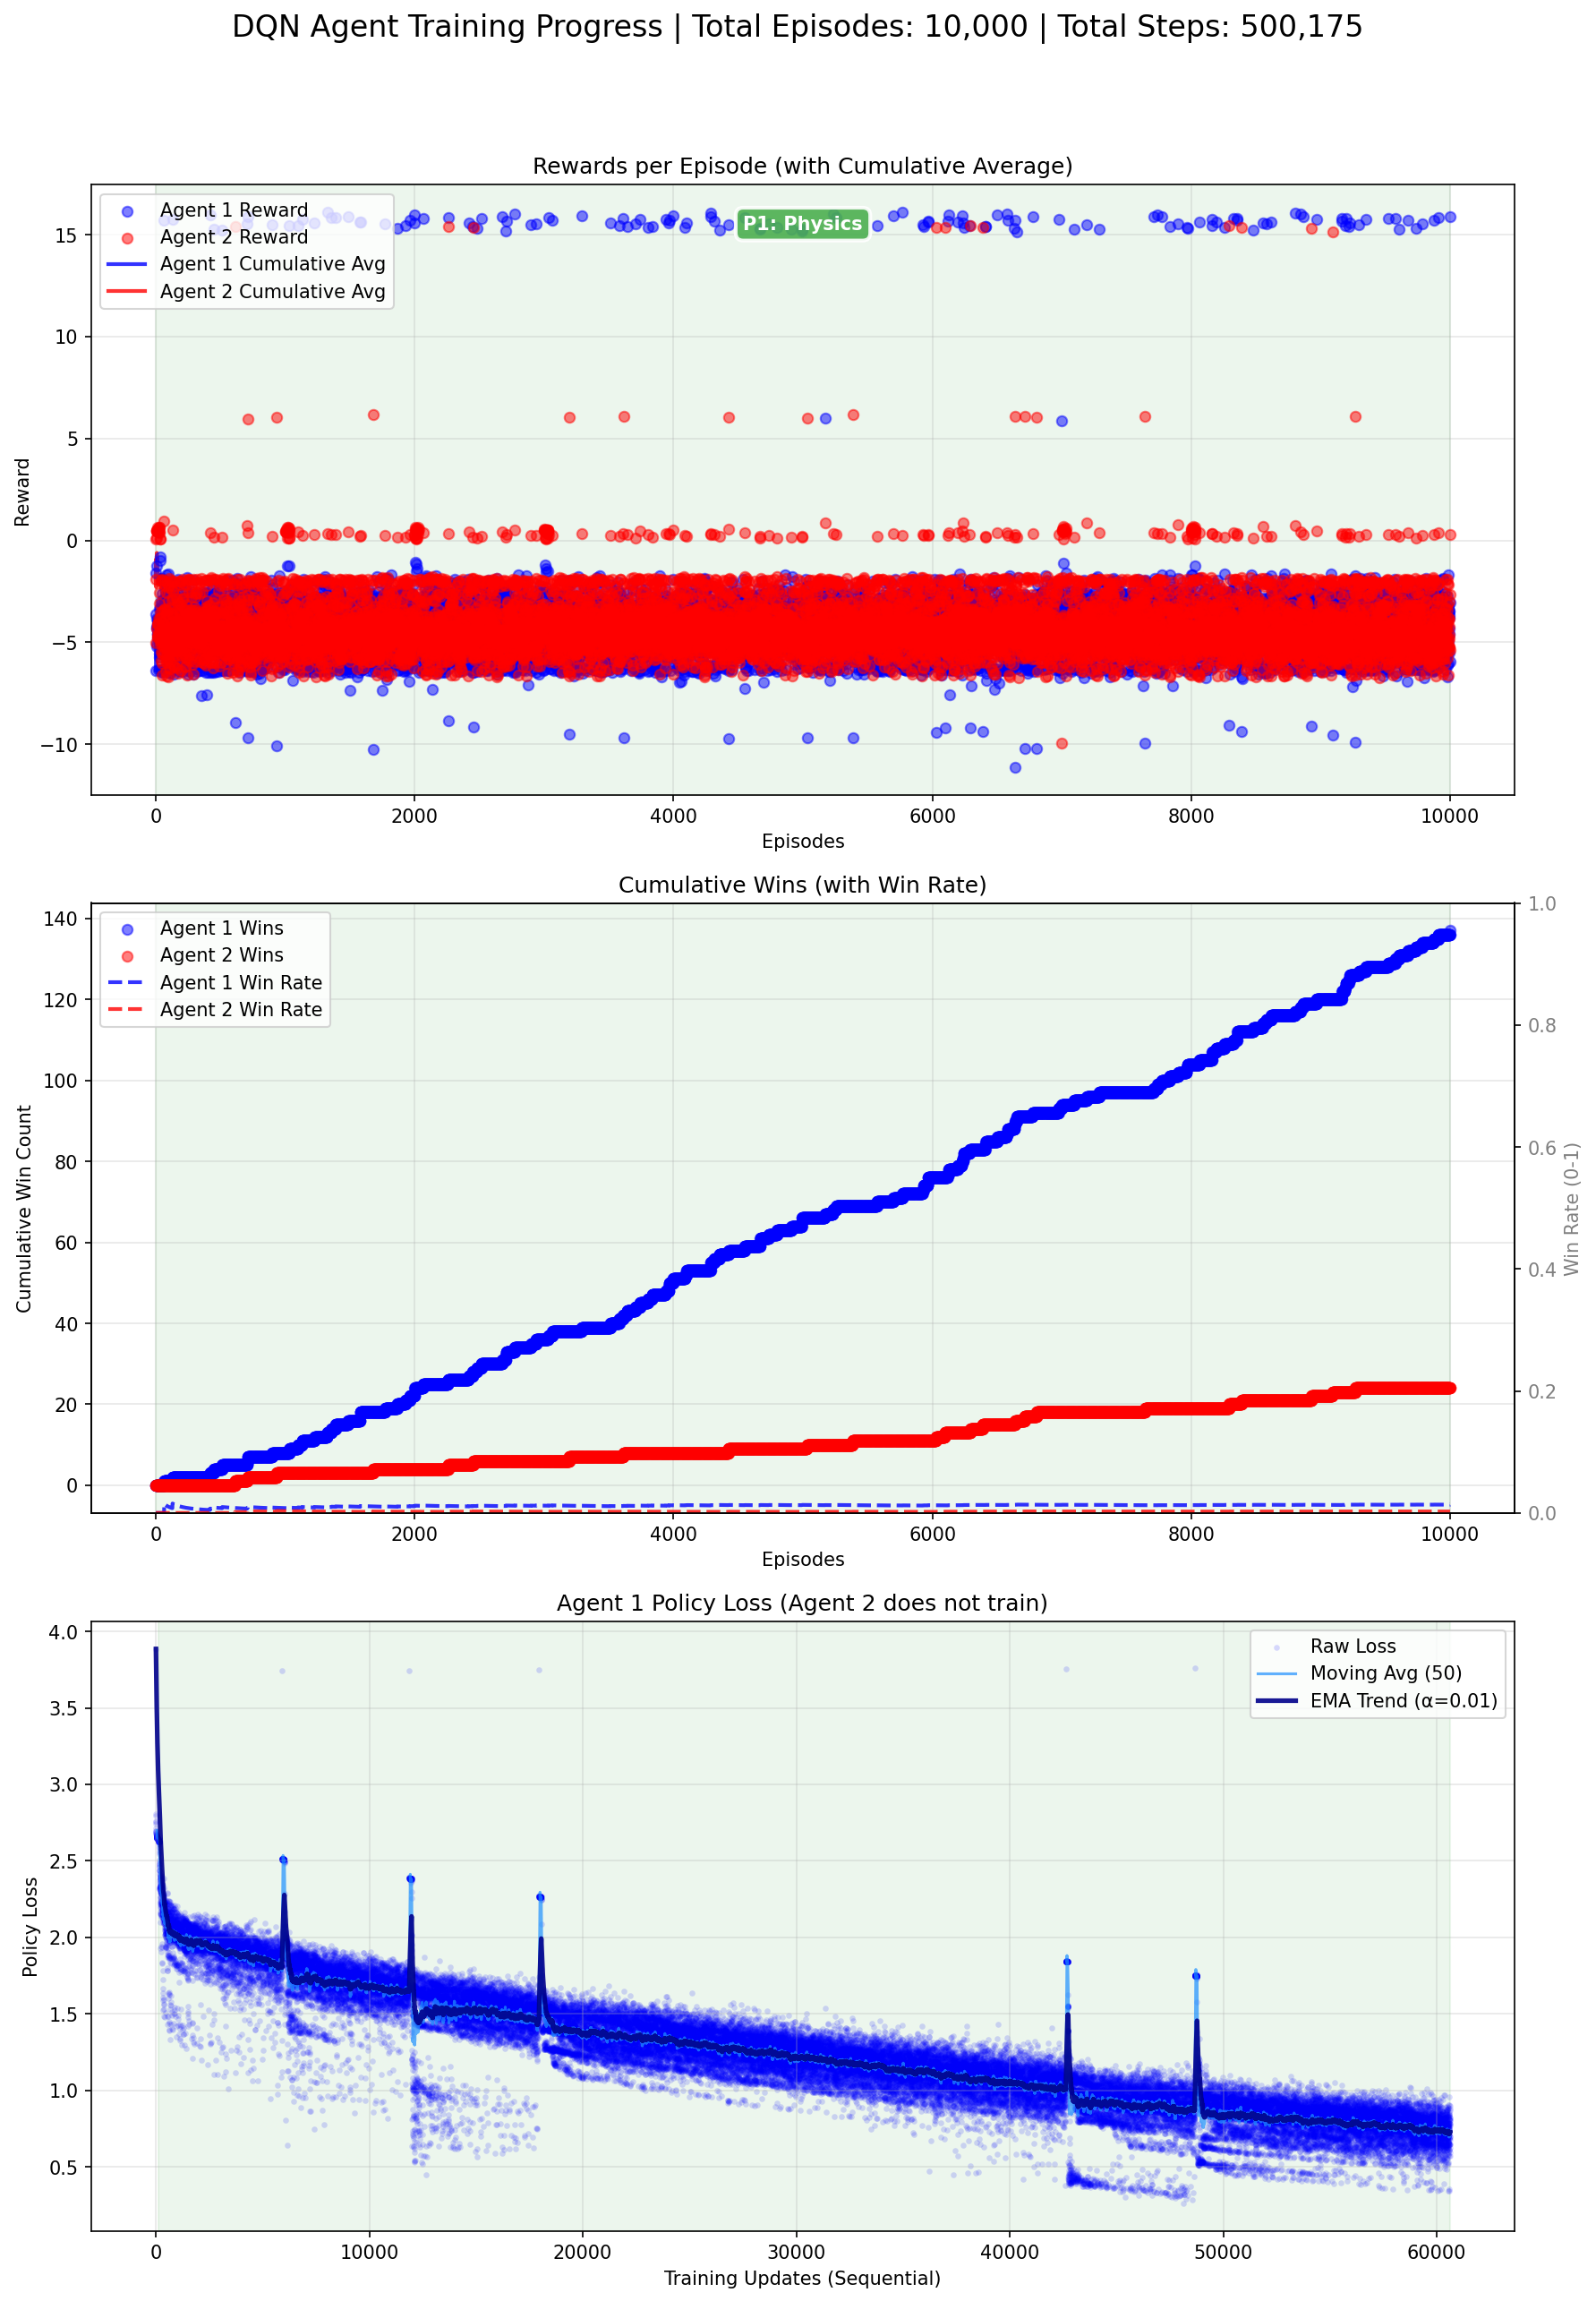
\includegraphics[width=0.9\textwidth,height=0.25\textheight,keepaspectratio]{figures/Results/training_progress_episode_10000.png}
    \caption{Training Progress: Episode 10,000}
    \label{fig:train_10k}
\end{figure}

\begin{figure}[ht]
    \centering
    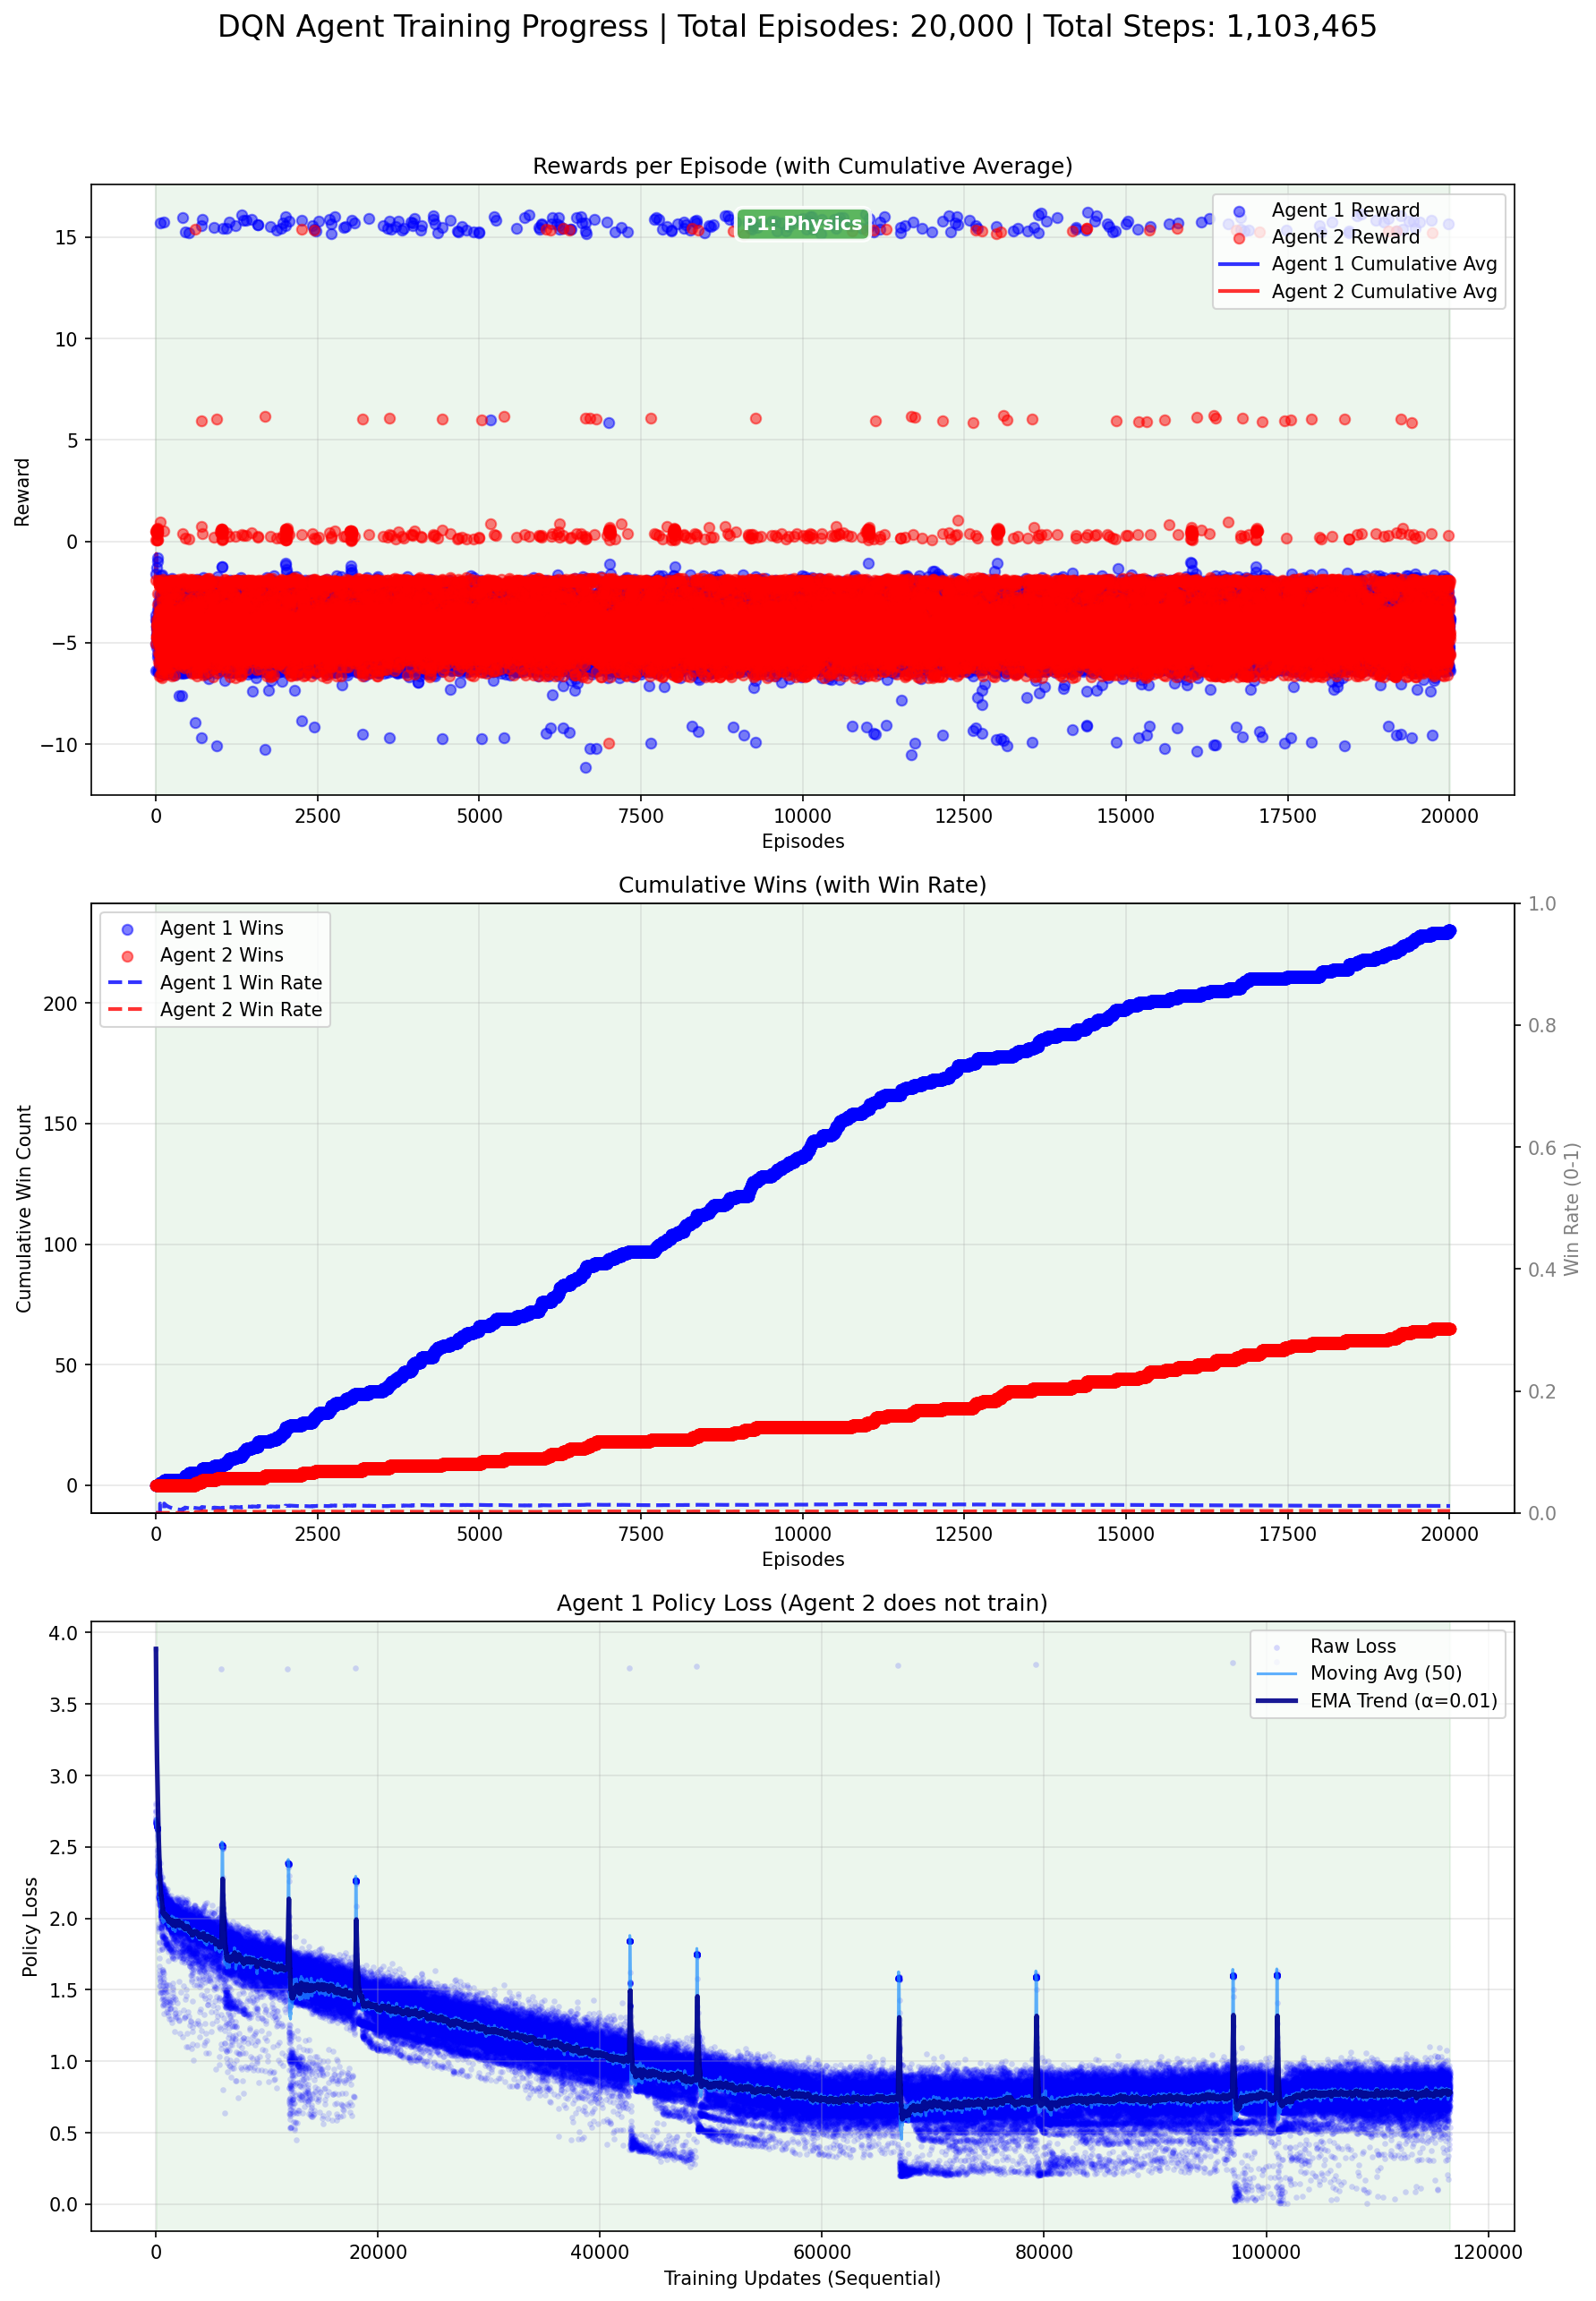
\includegraphics[width=0.9\textwidth,height=0.25\textheight,keepaspectratio]{figures/Results/training_progress_episode_20000.png}
    \caption{Training Progress: Episode 20,000}
    \label{fig:train_20k}
\end{figure}

\begin{figure}[ht]
    \centering
    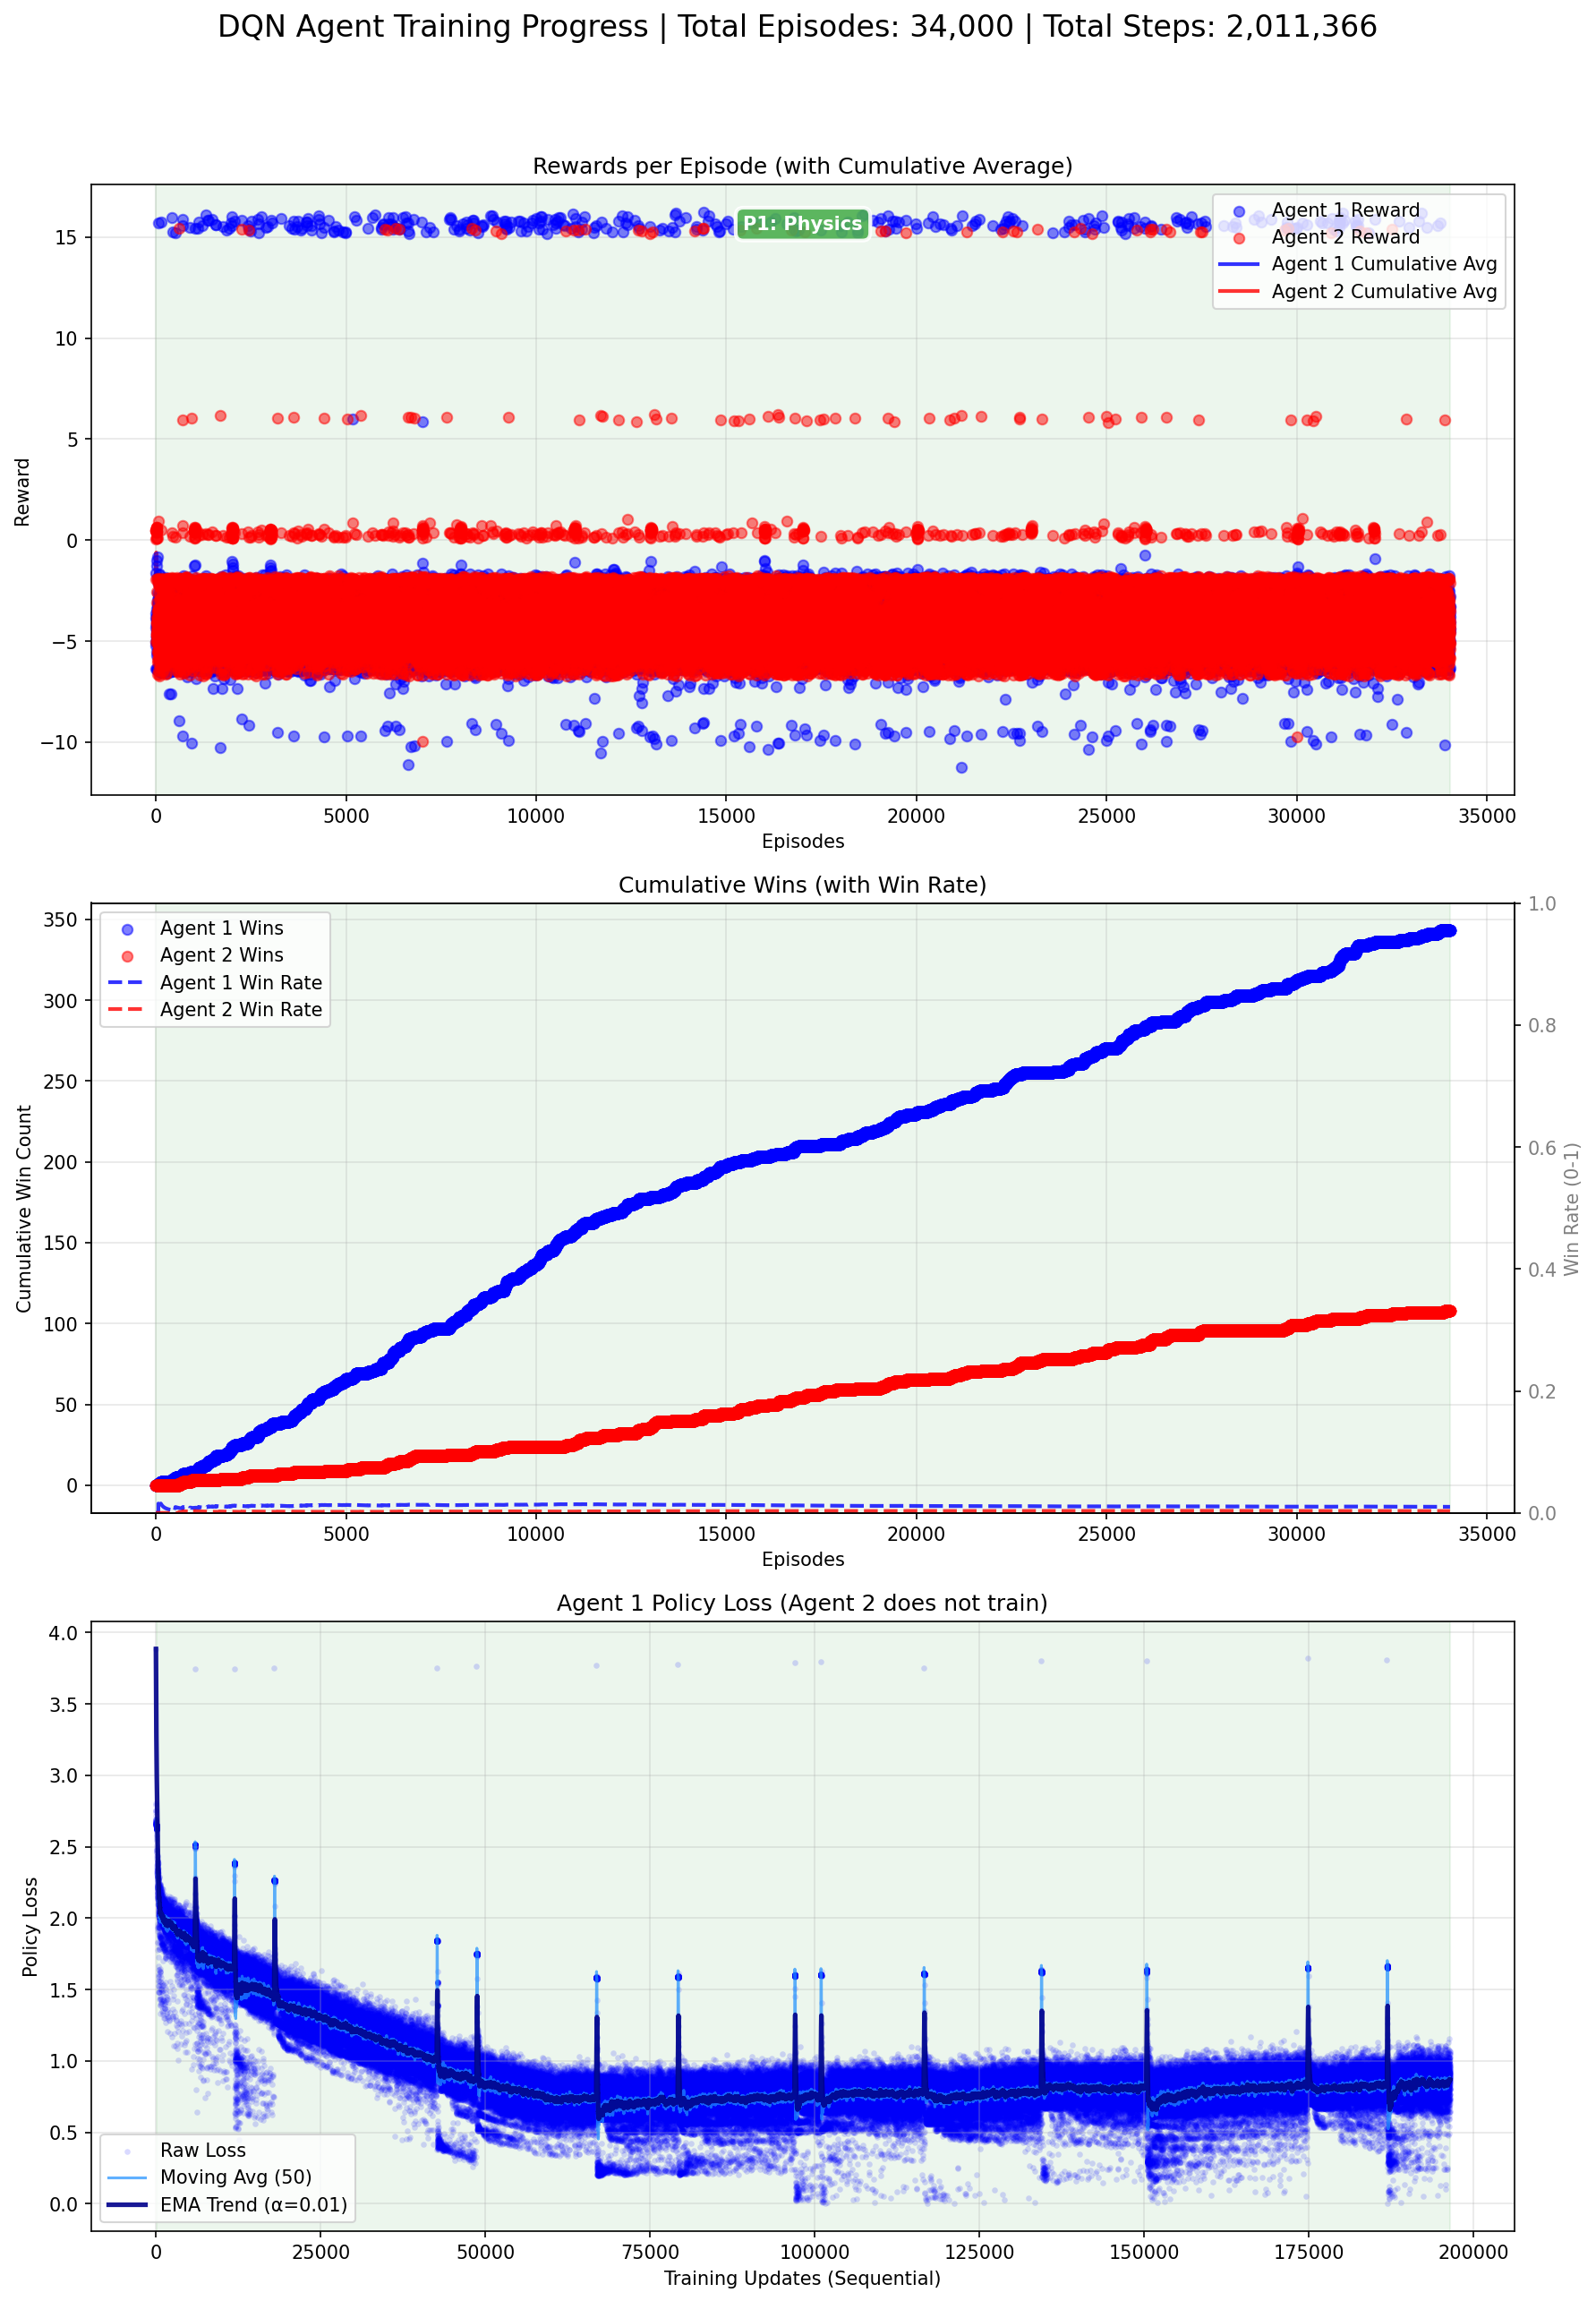
\includegraphics[width=0.9\textwidth,height=0.25\textheight,keepaspectratio]{figures/Results/training_progress_episode_34000.png}
    \caption{Training Progress: Episode 34,000}
    \label{fig:train_34k}
\end{figure}

\section{Discussion on Training Progress and Model Behavior}

The transition from early-stage exploration to the current 34,000-episode milestone reveals significant shifts in how the MARQ agent handles complex strategic interactions.

\subsection{Behavioral Evolution}
In early training (Episodes 0--5,000), the agent exhibited stochastic exploration with a high frequency of illegal move attempts and "indiscriminate charging," where high-value pieces like the Marshal were lost in routine skirmishes. By Episode 15,000, a clear shift towards tactical targeting emerged. The agent began to prioritize the capture of suspected lower-rank pieces while exhibiting defensive withdrawals when facing potential high-rank threats.

At the 34,000-episode mark, the model demonstrates "decisive targeting," specifically identifying and pursuing the opponent's flag once its location is inferred. However, this decisiveness is balanced by a "passive shuffling" tendency in common-value midgame states, where the agent avoids high-risk attacks to preserve material. This results in the observed draw-rate stabilization.

\subsection{Implicit Belief and AAREN Performance}
The Action-Augmented Recurrent Encoder (AAREN) has effectively learned to map action sequences to latent piece identities. As training progressed, the KL divergence between the predicted representation and ground truth revealed that the agent consistently identifies specialized units like Scouts (via multi-square movement) and Miners (via bomb engagement patterns) within 5--10 moves of their initial activity. This implicit deduced knowledge is what allows the Rainbow DQN to make calibrated risk assessments without explicit board information.

\subsection{Impact of Reward Overhaul}
The rescaling of rewards to $\pm 1.0$ for terminal states and the tightening of the C51 support to $[-10, +10]$ significantly improved the resolution of the distributional Q-values. Early training runs used a larger range which led to "clumping" of values, making it difficult for the agent to distinguish between marginally better moves. The current architecture allows for 0.4-unit resolution per atom, enabling the agent to better evaluate subtle positional advantages and territorial control rewards.

% %%%%%%%%%%%%%%%%%%%%%%%%%%%%%%%%%%%%%%%%%%%%%%%%%%%%%%%%%%%%%%%%%%%%%%%%%%%
% This file previously contained content from a different paper.
% The thesis conclusion is in recommendations.tex (Chapter: Conclusion and Recommendations).
%%%%%%%%%%%%%%%%%%%%%%%%%%%%%%%%%%%%%%%%%%%%%%%%%%%%%%%%%%%%%%%%%%%%%%%%%%% may also be used

%\appendix
%   \include{appendices/evaltool}
%   \include{appendices/reports}
%   \include{appendices/io}
%   \include{appendices/code}
%   \include{appendices/usersguide}

\nocite{*}
\bibliographystyle{acm}
{
\singlespace
\bibliography{references}
}

\begin{vita}


James Gabriel P. Mabagos is BS Computer Science student of the Department of Computer Science at the Ateneo de Naga University.
\\
\\
Mark Lawrence M. Quibot is BS Computer Science student of the Department of Computer Science at the Ateneo de Naga University.


\end{vita}

\end{document}
